\documentclass[a4paper,11pt]{article}
%\usepackage{bibtopic}
%\usepackage{natbib}
\usepackage{pgfplotstable}
\usepackage{float}
\usepackage{amsmath}
\usepackage{amssymb}
\usepackage{fullpage}
\usepackage{rotating}
\usepackage{tikz} \usetikzlibrary{trees}
\usepackage{pbox}
\usepackage{algorithm}
\usepackage[noend]{algpseudocode}
\usepackage{listings}
\usepackage{hyperref}
\usepackage{courier}
\usepackage{graphicx}
\usepackage{epsfig}
%\usepackage{cite}

\usepackage{siunitx}
\sisetup{per=slash, load=abbr}

\usepackage{tikz}
% \usetikzlibrary{calc,angles,positioning,intersections}
\usepackage{pgfplots}
\pgfplotsset{width=7cm, height=10cm, compat=1.4, every axis/.append style={thick}}

\newcommand{\AnyCond}[1]{\text{Any}(#1)}
\newcommand{\BoundedCond}[1]{\text{Bounded}(#1)}
\newcommand{\Constraint}[1]{\textsc{#1}}
\newcommand{\DepProps}{\textit{DepProps}}
\newcommand{\Distinct}{\Constraint{Distinct}}
\newcommand{\Failed}{\text{Failed}}
\newcommand{\FailedCond}[1]{\text{Failed}(#1)}
\newcommand{\FixedCond}[1]{\text{Fixed}(#1)}
\newcommand{\Fixpoint}{\text{AtFixpt}}
\newcommand{\NoneCond}[1]{\text{None}(#1)}
\newcommand{\Gecode}{\textit{Gecode}}
\newcommand{\GIST}{\textit{GIST}}
\newcommand{\Propagate}{\text{Propagate}}
\newcommand{\PropConds}[1]{\text{PropConds}(#1)}
\newcommand{\Sequence}[1]{\left[#1\right]}
\newcommand{\Set}[1]{\left\{#1\right\}}
\newcommand{\Subsumed}{\text{Subsumed}}
\newcommand{\Tuple}[1]{\left\langle#1\right\rangle}
\newcommand{\Unknown}{\text{Unknown}}

\pagestyle{empty}

\renewcommand{\thesection}{\arabic{section}}
\renewcommand{\thesubsection}{\arabic{section}.\arabic{subsection}}

\title{\textbf{Implementing Tuple Variables in Gecode\\
	Bachelor Thesis \\
    Uppsala University  \\
  }
}

\author{Patrik Broman}

\date{\today}


\begin{document}
\maketitle

\begin{abstract}

In constraint programming, efficient pruning is vital to avoid unnecessary searching. This thesis shows that tuple variables can be used to reduce the size of the search tree, which in turn reduces the execution time. The tuple variables are implemented in C++ for the Gecode library. The problem used to measure performance is finding paths through a deterministic finite automaton with different costs for each transition.
\end{abstract}

\setcounter{tocdepth}{2}
\tableofcontents
\pagestyle{plain}

\section*{Acknowledgements}
Thanks to Jean-No\"{e}l Monette and Pierre Flener for being helpful supervisors. \\
Thanks to Joseph Scott for helping me configuring Gecode. \\
Thanks to Johan Gustafsson for general help with C++. \\

\section{Introduction}
Constraint programming (CP) is a declarative style programming, and is very similar to solve equations in mathematics. A problem is modeled with variables, which must satisfy certain conditions. These conditions are called \textit{constraints}. The variables are initialized with a set of possible values. Such a set is called a \textit{domain}. The goal is to remove values from the domain until only one is left, and a state where all variables have a domain with only one value each is called a \textit{solution}.

When using CP it is often a problem that it is impossible to remove invalid combinations of values from the domains. Consider a problem where we have the variables $x$ and $y$. We initialize the domains $dom(x)=\{1,2,3,4\}$ and $dom(y)=\{3,4,5,6\}$. We also use the constraint $x=y$. In this case we can instantly remove 1 and 2 from $x$, and 5 and 6 from $y$. This leaves us with $dom(x)=\{3,4\}$ and $dom(y)=\{3,4\}$. Now, consider the same initial domains, but with the constraint $x\neq y$. We know that no solution has $x=y$, but we can not remove any value at all from any of the domains. 

Many CP problems could be solved more efficiently if it was possible to remove a combination of values from the variables, rather than removing the values individually. Recently, it was shown in a paper\cite{Monette771427} that a tuple variable can be used to link variables together. In this thesis, it is shown that it is possible to reach better performance by linking variables with tuples.

A \textit{tuple} is a mathematical object. It is an ordered list of elements. In this thesis a \textit{tuple variable} is a \textit{tuple} in Gecode, which in turn is a library for CP. Currently, Gecode supports boolean, integer, integer set and float variables. The tuple variable described here is an extension to the Gecode library.

To demonstrate that tuple variables can be used to increase performance, I have implemented two different variants of a tuple variable. Both of them are restricted to two dimensions. One of them keeps an exact representation of the domain, while the other approximates the second dimension by just storing the boundaries. Individual boundaries are stored for each value in the first dimension. I wrote propagators for these tuple variable implementations and a reference propagator to compare performance. Because the main purpose of this thesis is to show that tuple variables can improve performance I have intentionally avoided to optimize the code that handles the tuple variables. Even obvious and simple optimizations have been avoided. For the same reason I have optimized the reference propagator as far as I can, and I have also asked experienced CP-programmers for help with that.

To compare performance I used the tuple variables to find all valid strings for a deterministic finite automaton (DFA) with costs for each transition (cDFA). A cDFA does not only tell whether a string is accepted or not, but also the total cost for that particular string. The performance is measured by studying how the execution time and size of the search tree depend on four parameters: the number of states, the size of the alphabet, the maximum cost per transition and the size of the string.

The results confirm that tuple variables can be used to increase performance. The tuple variable which has an exact domain performs better than the one with an approximated domain. The latter one is almost identical to the reference. There is one case where the approximation is the best, and that is when the cost per transition is high. For most cases, the exact version is 80-100\percent faster than the integer version used for reference.



\section{Background}
\subsection{Constraint Programming}

Constraint programming (CP) is a method to solve problems by modeling the problem with variables and constraints that the variables must fulfill. The variables have an initial domain of possible values. Then \textit{propagators} are used to remove impossible values. Propagators are explained in detail in Section~\ref{sec:propagators}. CP is a \textit{declarative} type of programming, which basically means that the programmer states what is true. This is very much like mathematics. The \textit{constraints} work like equations.

A problem suitable for CP is a Sudoku. The most intuitive model is a $9\times9$ matrix of integer variables. The constraints are that all variables have a domain of $\{1,\ldots,9\}$, and that all variables in a row, column and box must be different. For a specific Sudoku constraints are added to require certain variables to have predetermined values.

When using CP, different variable types may be used. Gecode comes with boolean, integer, integer set and float variables. The available variable types limits the options to model a specific problem. With more different variables available, a specific problem can be modeled in different ways. For example, there is a problem called Eight queens\footnote{\url{https://en.wikipedia.org/wiki/Eight_queens_puzzle}}. The problem is to place eight queens on a chess board in such a way that no queen threatens another queen. If only boolean variables are available, the problem would have to be modeled with 64 boolean variables. With integer variables, 8 variables is sufficient. In the boolean case, each variable $b[i][j]$ would tell whether a tile has a queen or not, while in the integer variable case each variable $x[i]$ would tell on which row the queen in column $i$ should be placed on. By analyzing the Eight queen problem it is easy to realize that a solution must have one queen per column.

When no propagator can prune any values, a \textit{brancher} takes over. The brancher typically splits a variable into two parts: one with an assigned value and one with the rest of the domain, thus creating a search tree. After this branching, the propagators are called again for all branches. The branchers determine the structure of the search tree. Branchers are described in Section~\ref{sec:branchers}. 

Solving a CP-problem means alternating propagating and branching until some goal has been reached. The goal can, among others, be finding a solution, finding all solutions, or discovering that there are no solutions at all. The propagators have two main tasks. The most important task is to determine whether a \textit{solution} has been found or not. A \textit{solution} is a state where all variables are \textit{assigned}, which means their domain has been \textit{pruned} to the size of exactly one, and all propagators reports that the values assigned to the variables satisfies the constraints. A state where at least one variable has been pruned to size zero is called a \textit{failure}. The second task for a propatator is pruning. Pruning is when a propagator removes values from domains. A propagator does not necessarily be able to prune, but otherwise the branchers need to do all the work. In order to reach good performance, the propagators needs to prune as many values possible. For example, if a variable $x$ has a domain of $\{1..9\}$ and the constraint $x\le 4$ is used, a propagator could instantaneously remove the values $\{5..9\}$ from the domain.

Note that the domain of a variable never grows, and no values change. The only thing that happens to the domain after initialization is that values are removed by either a propagator or a brancher.

\subsection{Tuple}
In a mathematical context, a tuple is a finite length sequence (ordered list) of elements. The elements can be of any type, such as numbers, sets, and functions. The elements do not need to be of the same type. The most common type of tuples in mathematics and physics are vectors. Velocity and force are two examples. An $n$-dimensional tuple is called an $n$-tuple. In this thesis, a tuple is denoted by angle brackets. $\langle 3, 2, 1, 4, 2 \rangle$ is an example of a 5-tuple.

\subsection{Deterministic Finite Automaton}
A deterministic finite automaton (DFA) is a 5-tuple: $\langle Q,\Sigma,\delta,q_0, F\rangle$. $Q$ is a finite set of states. $\Sigma$ is called the alphabet, and is a finite set of symbols. $\delta : Q \times \Sigma \mapsto Q$  is a transition function, and maps a state and a symbol to a state. $q_0$ is called the starting state and is an element in $Q$. $F$ is a subset of $Q$, and these states are called accepting states. Any state from which there is no path (via one or more transitions) to an accepting state is commonly called a \textit{garbage state}. Furthermore, the set of garbage states are commonly viewed at as one state, called \textit{the} garbage state. Usually the garbage state is left out in both graphical and algebraic representations. 

A DFA \textit{consumes} symbols from a string from the beginning to the end. If the DFA is in an accepting state when all symbols in the string have been consumed the DFA \textit{accepts} the string. Figure~\ref{fig:dfasdp} shows a 2-state DFA with omitted garbage state.

\begin{figure}[H]
\centering
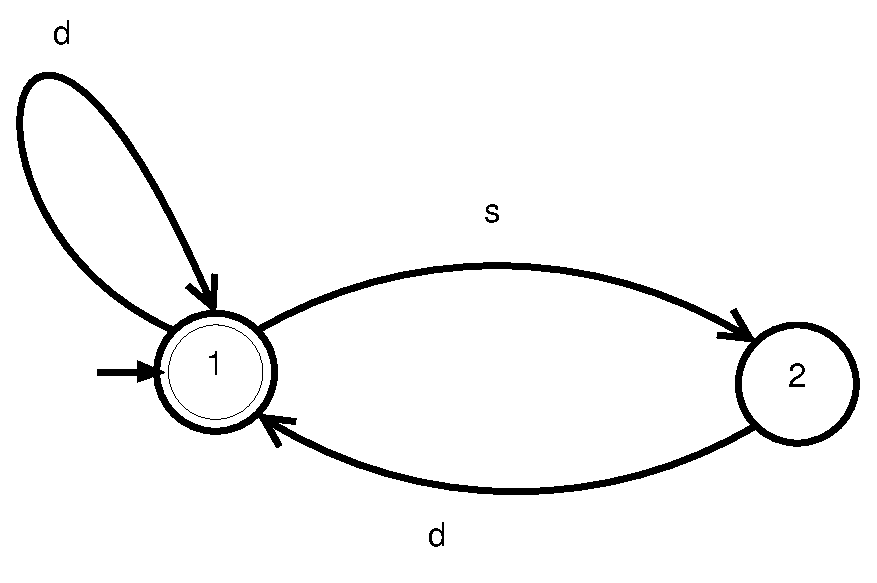
\includegraphics[scale=0.6]{dfa.eps}
\caption{A DFA for the Swedish drinking protocol, as it is showed in the Gecode documentation\cite{mpg}. State $1$ is the starting state and the only accepting state. State $2$ is a non-accepting state. The symbols $d$ and $s$ denotes drinking and singing. The DFA means that you may drink whenever you want, but if a song has been sung you have to drink before you leave. The regular expression for this DFA is $(d|sd)^{*}$}
\label{fig:dfasdp}
\end{figure}

A finite automaton where $\Sigma$ maps a state and a symbol to a set of states instead of a single state is called a nondeterministic finite automaton (NFA). Another way to define it is allowing empty string-transitions (transitions that do not consume a symbol). These transitions are denoted $\epsilon$. It is common to also allow an NFA to have multiple starting states. NFA:s and DFA:s are mathematically equivalent. Every NFA can be converted to a DFA and vice versa. The conversion from NFA to DFA is easily done with a method called \textit{powerset construction}. An NFA is typically smaller, and is often easier to construct than a corresponding DFA.

DFA:s (and therefore also NFA:s) are closely related to regular expressions (regex). Every regex corresponds to a DFA and vice versa. Note that this is not true for the extended regexes one can find in many languages, such as Perl and Python. A pure regex can be written with the operators $($,$)$,$|$ and $^{*}$. One example that uses all of them is $ab(a|b)c^{*}$ which is a regex for the language of all strings starting with $ab$, continuing with either an $a$ or a $b$, and ends with zero or more $c$. A corresponding DFA for this regex is $Q=\{1,2,3,4\}, \Sigma=\{a,b,c\}, q_0=1, F=\{4\}, \delta(1,a)=2, \delta(2,b)=3, \delta(3,a)=4, \delta(3,b)=4, \delta(4,c)=4$. Any other parameters for $\delta$ returns the garbage state. One practical implication of this definition is that a pure regex can not check for matching parenthesises in a string.

In this thesis an extended version of a DFA, a counting DFA (cDFA), is used. The difference is that the state function not only maps a state and a symbol to a state, but to a tuple of both a state and a cost. Another possible approach is to define the DFA as a 6-tuple with an added cost function. Mathematically the two approaches are equivalent. When displayed graphically the first approach is more suitable, but for implementation related reasons the latter one is used in the actual code. Figure~\ref{fig:cdfasdp} shows an example of an cDFA.

In the paper Propagating Regular Counting Constraints cDFA means \textit{counting DFA}. It is defined in a similar manner, and counting can be interpreted as cost. Whenever a DFA is mentioned in this thesis, it is a cDFA.

\begin{figure}[H]
\centering
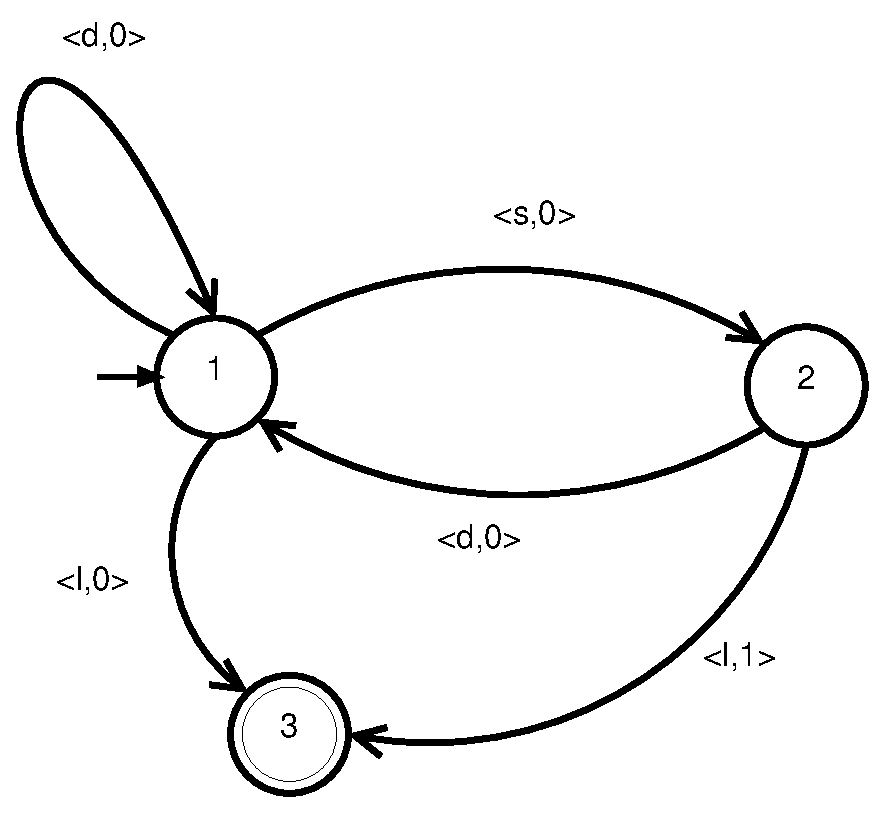
\includegraphics[scale=0.6]{cdfa.eps}
\caption{A cDFA for the Swedish drinking protocol. It is an altered variant of the DFA shown in Figure~\ref{fig:dfasdp}. The symbols $d$ and $s$ still means drinking and singing, but the symbol $l$ is introduced for leaving. Also, costs are introduced for each transition, so you can leave without drinking after singing, but with some kind of cost.}
\label{fig:cdfasdp}
\end{figure}

\subsection{Motivation for Tuple Variables}
When solving a problem with CP, it is desirable to minimize the search tree to avoid brute force searching. The size of the search tree depends on the model and the propagators. With good models and propagators the variable domains can be pruned to smaller sizes, keeping the branching and searching to a minimum. For example, if two variables $x$ and $y$ have domains $dom(x)=\{1,2,3\}$ and $dom(y)=\{2,3,4\}$, and the constraint $y<x$ is applied, then the domains can be pruned to $dom(x)=\{3\}$ and $dom(y)=\{2\}$ in one step, and this is the solution to the problem. If we instead have the same variables and domains but instead use the constraint $x\neq y$, nothing can be pruned, since for all values in both domains there exists solutions. 

In this example, the problem was modeled with two integer variables. If the problem would be modeled with one tuple variable instead of two integer variables, pruning would be possible. Then we would have a tuple variable $t$ with domain 
$dom(t)=\{
\langle1,2\rangle,\allowbreak 
\langle1,3\rangle,\allowbreak 
\langle1,4\rangle,\allowbreak
\langle2,2\rangle,\allowbreak
\langle2,3\rangle,\allowbreak
\langle2,4\rangle,\allowbreak
\langle3,2\rangle,\allowbreak
\langle3,3\rangle,\allowbreak
\langle3,4\rangle\}$ 
and pruning with the same constraint would yield 
$dom(t)=\{
\langle1,2\rangle,\allowbreak
\langle1,3\rangle,\allowbreak
\langle1,4\rangle,\allowbreak
\langle2,3\rangle,\allowbreak
\langle2,4\rangle,\allowbreak
\langle3,2\rangle,\allowbreak
\langle3,4\rangle\}$. 
This shrinks the size of the search tree from 9 to 7. 

If we instead look at the case where $dom(x),dom(y)=\{1,\ldots,1000\}$ and the constraint $x=y+1$ the benefits are more obvious. Using integer variables, only the values $x=1$ and $y=1000$ can be pruned. If tuple variables are used, the size of the domain would shrink from $10^6$ to $10^3$. This indicates that tuple variables can be quite useful. Note though that these two examples are selected because they are easy to understand, and in reality the performance would probably drop if tuple variables were used for them. A more realistic example is the constraint $DFA(state_1, cost_1, state_0, cost_0, symbol, statefun, costfun)$. It is a constraint for a DFA with costs and a solution has to satisfy $state_1= statefun(state_0, symbol)$ and $cost_1=cost_0+costfun(state_0, symbol)$. This is the constraint used in this thesis. Furthermore, the constraint is linked in several steps: $DFA(state_n, cost_n, state_{n-1}, cost_{n-1}, symbol_{n-1}, statefun, costfun)$. A solution to this problem would be three arrays: one for states, one for costs, and one for symbols. With tuple variables, this could be done more efficiently by combining states and costs into one variable: $DFA(P, Q, symbol, statefun, costfun)$ where $P=\langle state_1, cost_1\rangle$ and $Q=\langle state_0, cost_0\rangle$.

The main benefit of a tuple variable is the possibility to link variables together. The most intuitive case is when dealing with coordinates, since a coordinate is a tuple by definition, but it can be generalized to any case where it is interesting to see if a combination of two or more values is a part of a solution. 

\subsection{Creating a Custom Variable in Gecode}
Gecode is an open source CP solver programmed in C++ and is licensed under the MIT license. It is flexible and supports customization of most parts, including variable types, branchers and propagators. It is suitable for both education and professional use. In this thesis, Gecode 4.3.2 is used. This version is no longer available. However, version 4.3.3 should work. For more information, visit the homepage. \url{http://www.gecode.org}

Everything that follows in this section is a summary of Chapter P, B, and V in Modeling and Programming with Gecode\cite{mpg}. 

When implementing a new variable in Gecode, there are several things that should be written. Among them is a specification file, various classes and propagators.
\subsubsection{Specification File}\label{sec:specfile}
Creating the specification file is the first thing that needs to be done when designing a new variable.  A simple specification file could look like this:

\begin{figure}[H]
\begin{minipage}{\linewidth}
\begin{lstlisting}[frame=single]
[General]
Name:        IntTuple
Namespace:   MPG::IntTuple
[ModEvent]
Name:        FAILED=FAILED
[ModEvent]
Name:        VAL=ASSIGNED
[ModEvent]
Name:        NONE=NONE
[PropCond]
Name:        NONE=NONE
[PropCond]
Name:        VAL=ASSIGNED
ScheduledBy: VAL
[End]
\end{lstlisting}
\end{minipage}
\caption{A minimal specification file.}
\end{figure}

There are three different sections in the file. The specification file must start with the [General] section and end with [End]. There are also sections for modification events and propagation conditions. The specification file is used by a configuration script to generate a base class, from which the variable implementation class will inherit.

The [General] section is trivial. This is where the name and namespace of the variable are specified. Both name and namespace are arbitrary. In Gecode the standard variables have namespace Gecode::VarName and in the examples in the documentation they instead have the namespace MPG::VarName.

The [ModEvent] section specifies the modification events. The modification events describes how the variables change. When a propagator wants to prune the domain for a variable, it uses the class methods that the variable implementation provides. It does not modify the domain directly. If no values are pruned, then the variable returns the modification event NONE, and if all values are pruned then it returns FAILED. When the domain of a variable gets pruned so that exactly one element remains, then ASSIGNED is returned. For all variables, modification events for NONE, FAILED, and ASSIGNED are required. More modification events may be added to avoid unnecessary executions of propagators. For example, the modification event BND can be used when only the boundaries of a domain has changed. Note that other names than the required ones are arbitrary. DOM is usually denoting when any change has been made.

The [PropCond] section describes how the propagators are scheduled, depending on how the variables have changed. For all variables, propagator conditions for NONE and ASSIGNED are required.

\subsubsection{Variable Implementation}
The variable implementation class would with the specification file in the previous section be called IntTupleVarImp and inherit from the class IntTupleVarBase generated from the specification file. It has to implement a function called \texttt{assigned} that returns true iff the variable is assigned. The implementation class is the class that does all the work. This is where the modification events are defined, and the modification events are the only methods that directly changes the domain. The implementation class implements both the getters and setters that are used by the variable class and view classes.

\subsubsection{Variable Class}
The variable class is the class that is used when modeling the actual problem and inherits from the variable implementation. It is a read-only interface, and a programmer that does not program any custom branchers or propagators will not use anything else than this. This class would be called IntTupleVar by convention.

\subsubsection{Deltas}
Deltas are used for passing information about changes to improve efficiency. In this thesis an empty class is used. The only reason it is defined at all is that some mandatory virtual functions takes Deltas as arguments.

\subsubsection{Views}
The variable implementation class implements methods for modification of the variable, but the variable class does not give access to these. Instead these are called from a view, which is a read and write interface to the implementation class.

\subsubsection{Propagators}
\label{sec:propagators}
A propagator implements constraints and prunes variables. It interacts with the views, and \textit{subscribes} to variables. A propagator should subscribe to all variables it depends on. When a propagator has subscribed to a variable, it receives information whenever the domain of that variable changes. For instance, a propagator for the constraint $x\le y$ should subscribe to the maximum value of x and minimum value of y, because if none of these changes, then there is nothing the propagator can do. Subscriptions is done to the view classes. A propagator class must have the following methods:
\begin{itemize}
\item{post} - The method for posting a constraint, which basically is declaring that a certain constraint should be used.
\item{dispose} - This works as a destructor. The only reason Gecode does not use regular destructors is that destructors in C++ can not take arguments.
\item{copy} - A method to copy the propagator.
\item{cost} - Estimates the cost to run the propagator. This does not affect the correctness, but may improve efficiency by making it easier for the Gecode engine to schedule cheap propagators before expensive ones.
\item{propagate} - The method which does the actual work. It prunes domains and determines the status to return.
\end{itemize}
The propagate method has the following possible return values:
\begin{itemize}
\item{ES\_FAILED} - There is no combination of values in the domains that satisfies the constraint. 
\item{ES\_FIX} - The propagator is at a fixpoint. It is impossible for the propagator to prune more values before a domain has changed for any of the variables the propagator has subscribed to. This can be done by either a brancher or another propagator.
\item{ES\_NOFIX} - The propagator may be at a fixpoint, but it is not guaranteed. Running it once more may or may not prune some values. 
\item{ES\_SUBSUMED} - The propagator is done. Regardless of any changes made to the variables, this particular propagator will not be able to do anything more.
\end{itemize}
The propagator must be able to return ES\_FAILED and at least one of the others. ES\_NOFIX is safe to return in the sense that it does not promise anything. If it can't be guaranteed that the propagator has reached a fixpoint, this should be returned. 

\paragraph{Consistency}
A propagator can work with different consistencies. Bound consistency means that the propagator ensures that the bounds (min and max value for an integer variable) satisfies the constraint. If $dom(x)=\{1,5,7,8\}$ and $dom(y)=\{1,3,7\}$ and the constraint $x=y$ is applied, the propagator would yield $dom(x)=\{1,5,7\}$ and $dom(y)=\{1,3,7\}$ with bounds consistency, since there are solutions to $x=1$, $x=7$, $y=1$ and $y=7$. $x=5$ and $y=3$ is not considered. If the same constraint were applied with domain consistency we would end up with $dom(x)=\{1,7\}$ and $dom(y)=\{1,7\}$. Pruning with domain consistency does in general cost more execution time, but results in a smaller search tree.

\subsubsection{Branchers}
\label{sec:branchers}
When there are no propagators able to prune any variables, searching is performed. The branchers determines the structure of the search tree. The simplest brancher just puts the first value in the first branch and the rest of the values in a second branch. Another way is to pick a random value in the domain, but more sophisticated ways exist. A brancher can create an arbitrary number of nodes, but the union of all nodes must be the original domain, and at least one node must be different from the others. Ideally, the intersection between two nodes created by a brancher is empty.

For the variables created for this thesis, only a simple brancher is implemented. The domain of IntPairVar is a long sorted list, and the brancher picks the first value. However, it is not used. See Section~\ref{sec:performancetest} for details. A brancher is not strictly needed to implement a variable, but if there is no brancher the propagators must be able to prune the variables to a solution or a failure. Otherwise it is required. 

\section{The IntPairVar Variables}
To keep things simple, only two-dimensional integer tuples (Pairs) are considered. The specification files are kept almost as minimal as described in Section~\ref{sec:specfile}. Both implementations use identical specification files, except for the name of the variable. 

Two variants are implemented. One stores an exact representation of the domain, while the other stores an overapproximation. This means that the domain is bigger than it should be. The domain still fulfills the condition that it contains all values that should, but also some values that it should not. An approximation saves some memory, but the biggest benefit is that some operations can be done in constant time. The approximate version only stores the boundaries for the second dimension. It stores separate boundaries for each value in the first dimension. A more detailed description is found in Section~\ref{sec:impapprox}. Now, consider the case with a tuple $t$ and the constraint $t.x\neq5$. The exact version has to remove an arbitrary amount of elements. The approximate version only needs to remove one element. 

The drawback with the approximation is that it can not be pruned as efficiently as an exact representation. This is demonstrated below in Figure~\ref{fig:pair}.

\begin{figure}[H]
  \centering
  \pgfplotsset{
    scale only axis,
%    xmin=1,
  }
  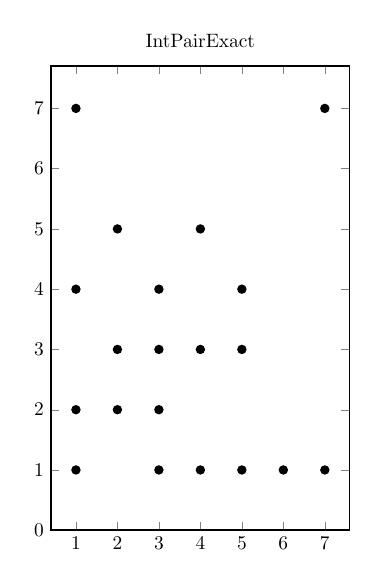
\begin{tikzpicture} [scale=0.7]
    \begin{axis}[
        title=IntPairExact,
        xtick=data,
        ymin=0,
      ]
      \addplot[black, mark=*, only marks]
       plot coordinates
       {  
       (1,1)       (3,1) (4,1) (5,1) (6,1) (7,1)
       (1,2) (2,2) (3,2) 
             (2,3) (3,3) (4,3) (5,3)
       (1,4)       (3,4)       (5,4)
             (2,5)        (4,5) 
       (1,7)                               (7,7)
       }; 
    \end{axis}
  \end{tikzpicture}
  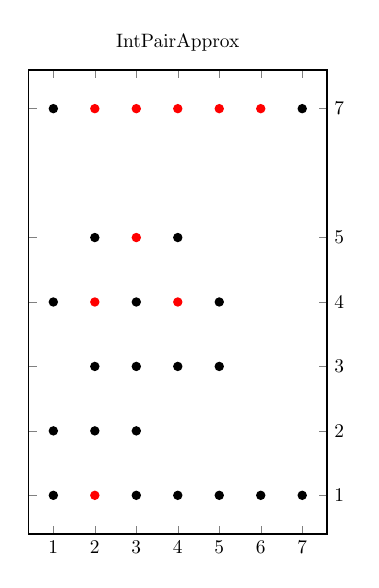
\begin{tikzpicture} [scale=0.7]
    \begin{axis}[
        yticklabel pos=right,
        xtick=data,
        title=IntPairApprox,
        ytick=data
        ]
      \addplot[black, mark=*, only marks]
       plot coordinates
       {  
       (1,1)       (3,1) (4,1) (5,1) (6,1) (7,1)
       (1,2) (2,2) (3,2) 
             (2,3) (3,3) (4,3) (5,3)
       (1,4)       (3,4)       (5,4)
             (2,5)        (4,5) 
       (1,7)                               (7,7)
       }; 
      \addplot[red, mark=*, only marks]
       plot coordinates
       {  
             (2,1) 
       


                  (2,4)    (4,4)
                       (3,5)
            (2,7) (3,7) (4,7) (5,7) (6,7)
       }; 

    \end{axis}
  \end{tikzpicture}

 \caption{Comparasion between IntPairExact and IntPairApprox representing the same domain. The red dots are values that should not be there, but IntPairApprox only stores the boundaries for the second dimension.}\label{fig:pair}
\end{figure}



The same benefit also holds for the following example: First we define a constraint $YLTIXEQ$ (y less then if x equal) such that $YLTIXEQ(p, y, x)$ means that $p.x=x\implies p.y<y$. With the exact variant there are possibly several values that needs to be removed. The approximate version only needs to change the value of the higher bound for the element with x-value $x$.

Class names follows the convention in Gecode. The variable classes are therefore named IntPairExactVar and IntPairApproxVar. When something is mentioned that is not specific for either the exact or the approximate variant, the name IntPairVar is used. Note that although the names ends with "Var" it is not necessarily the variable class that is referenced, but the variable as a whole. The built in integer variable that comes with Gecode has the name IntVar.

There are three things added to the specification file described in Section~\ref{sec:specfile}. The first two is the DOM modification event and the propagator condition. These are used to schedule the propagators. As soon as the domain of any variable is changed, all propagators that have subscribed to that variable will be scheduled to run again. The last change to the specification file is the line \texttt{Dispose: true}. This is needed when using external memory resources outside Gecode. The domains are stored as vectors from the C++ standard library, and therefore dispose is required. The way Gecode is designed, the destructors for variables are never called. If a variable needs a destructor it needs to be replaced by a method called \texttt{dispose}. This method explicitly calls \texttt{vector::$\sim$vector()}, which is the destructor for \texttt{vector}.

\begin{figure}[H]
\begin{minipage}{\linewidth}
\begin{lstlisting}[frame=single]
[General]
Name:           IntPairApprox
Namespace:      MPG::IntPairApprox
Dispose:        true
[ModEvent]
Name:           FAILED=FAILED
[ModEvent]
Name:           NONE=NONE
[ModEvent]
Name:           VAL=ASSIGNED
Combine:        VAL=VAL
[ModEvent]
Name:           DOM=SUBSCRIBE
Combine:        VAL=VAL, DOM=DOM
[PropCond]
Name:           NONE=NONE
[PropCond]
Name:           VAL=ASSIGNED
ScheduledBy:    VAL
[PropCond]
Name:           DOM
ScheduledBy:    VAL, DOM
\end{lstlisting}
\end{minipage}
\caption{The specification file for IntPairApproxVar. The specification file for IntPairExactVar is equal, except for name and namespace.}
\end{figure}

The main purpose of this thesis is to show that tuple variables have benefits over regular IntVar variables for certain problems. For that reason the code for IntPairs has purposely been kept unoptimised. For example, the modification events implemented in the variable implementation do not use the fact that the domains are sorted. Just fixing this would decrease the time complexity from linear to logarithmic for operations like removing a value from a domain. This would be especially efficient when removing ranges of values. Currently, they are removed one by one.

The complete source can be found at \url{http://www.github.com/klutt/gecode-tuples}

\subsection{Implementation of IntPairExactVar}
The exact version does not approximate the domain, that is, the implementation is a long list of all integer pairs that are currently in the domain. The domain is stored as \texttt{std::vector<struct \{int x, int y\}>}. 

\paragraph{Modification Events}
\begin{itemize}
\item {\textbf{nq(Pair p) - }} Remove p from domain. $\mathcal{O}(n)$ where $n$ is number of elements in the domain.
\end{itemize}

\paragraph{Other methods}
\begin{itemize}
\item {\textbf{contains(Pair p) - }} Returns true if the domain contains p, and false otherwise. $\mathcal{O}(n)$ where $n$ is number of values in the domain.
\end{itemize}

\subsection{Implementation of IntPairApproxVar}
\label{sec:impapprox}
This version of IntPairVar approximates the domain by just storing one dimension exactly. For the other dimension, only the boundaries are stored. Unique boundaries are stored for each value in the first dimension. The benefits are less use of memory and faster calculations for some operations, but the drawback is that the domain can not be pruned as efficient as the exact version, because no values whose y-value is between the bounds can be pruned. The domain is stored as \texttt{std::vector<struct\{int x, int y\_low, int y\_high\}>}

\paragraph{Modification Events}
\begin{itemize}
\item {\textbf{nq(Pair p) - }} Remove p from domain. $\mathcal{O}(n)$ where $n$ is the number of different x-values in domain.

\item{\textbf{yeqforspecificx(PairInterval p) - }} Remove all values from domain whose y-value is not in the interval $[p.ylow; p.yhigh]$ iff those values x-values is equal to $x$. $\mathcal{O}(n)$ where $n$ is the number of different x-values in domain. In the actual source code the name xeq is used, which is a bad name. The definition of this modification event was altered during development, but the name was never changed.

\item{\textbf{xeq(vector\textless Pair\textgreater v) - }} Remove all values from domain whose x-value does not exist in $v$. $\mathcal{O}(nm)$ where $n$ is number of x-values in domain and $m$ is number of elements in $v$.
\end{itemize}

\paragraph{Other methods}
\begin{itemize}
\item {\textbf{contains(Pair p) - }} Returns true if the domain contains p, and false otherwise. $\mathcal{O}(n)$ where $n$ is number of different x-values in the domain.
\end{itemize}

\subsection{Implementation of DFA Propagators}
The DFA \textit{propagators} are the actual implementations of the DFA \textit{constraint}. These propagators are implemented in three different ways. Two propagators are for IntPairVar and one is for IntVar variables. The latter one is only for reference when comparing performance. The algorithms for the propagators are described below in pseudo code.

All three implementations work in a similar manner. $PreState$ and $PreCost$ is domains containing current state and accumulated cost so far in the DFA. $PostState$ and $PostCost$ is the result of reading the symbol in $Symbol$. Since the Pairs makes it possible to bundle cost and state to a single variable, they are just called $Pre$ and $Post$. The basic principle is: for all symbols and all states in $Pre$, calculate the possible values for $Post$. Remove everything from $Post$ that is not reachable from any element in $Pre$. If nothing is reachable from a certain $Pre$, also remove that element from $Pre$. This is done by creating lists containing all elements that should remain in the domains, and then removing everything from the domains that is not in those lists.

%Int
\begin{figure}[H]
\begin{algorithm}[H]
\caption{DFA propagator IntVar\newline $\mathcal{O}(\#(PostState)\#(PostCost)\#(PreState)\#(PreCost)\#(Symbol))$}
\begin{algorithmic}[1]
\Procedure{DFAprop}{IntVar PostState, IntVar PostCost, IntVar PreState, IntVar PreCost, IntVar Symbol, Statefunction S, Costfunction C}
\State Intdomain newPostState, newPreState, newPostCost, newPreCost, newSymbol := $\emptyset$
\ForAll {symbol in Symbol}
	\ForAll {preState in PreState}
		\State int state := S(pre.state, symbol)
		\If {PostState.contain(state) and p.state $\neq$ garbage state}
					\State newPostState := newPostState $\cup$ state
			\State newPreState := newPreState $\cup$ pre
			\State newSymbol := newSymbol $\cup$ symbol 
			\ForAll {cost in PreCost}
				\State int postCost := cost + C(preState, symbol)
				\If {PostCost.contains(postCost)}
					\State newPreCost := newPreCost $\cup$ cost
					\State newPostCost := newPostCost $\cup$ postCost
				\EndIf
			\EndFor
		\EndIf
	\EndFor
\EndFor
\State PostState := PostState $\cap$ newPostState
\State PreState := PreState $\cap$ newPreState
\State PostCost := PostCost $\cap$ newPostCost
\State PreCost := PreCost $\cap$ newPreCost
\State Symbol := Symbol $\cap$ newSymbol
\EndProcedure
\end{algorithmic}
\end{algorithm} 
\caption{Propagator for DFA constraint for IntVar variables}\label{fig:algint}
\end{figure}

%Exact
\begin{figure}[H]
\begin{algorithm}[H]
\begin{algorithmic}[1]
\Procedure{DFAprop}{IntPairVar Post, IntPairVar Pre, IntVar Symbol, Statefunction S, Costfunction C}
\State Pairdomain newPost, newPre := $\emptyset$
\State Intdomain newSymbol := $\emptyset$
\ForAll {symbol in Symbol}
	\ForAll {pre in Pre}
		\State Pair p := (S(pre.state, symbol), pre.cost+C(pre.state, symbol))
		\If {Post.contain(p) and p.state $\neq$ garbage state}
			\State newPost := newPost $\cup$ p
			\State newPre := newPre $\cup$ pre
			\State newSymbol := newSymbol $\cup$ symbol 
		\EndIf
	\EndFor
\EndFor
\State Post := Post $\cap$ newPost
\State Pre := Pre $\cap$ newPre
\State Symbol := Symbol $\cap$ newSymbol
\EndProcedure
\end{algorithmic}
\caption{DFA propagator IntPairExact \newline $\mathcal{O}(\#(Post)\#(Pre)\#(Symbol))$}
\end{algorithm}
\caption{Propagator for DFA constraint for IntPairExactVar variables}\label{fig:algexact}
\end{figure}
%Approx
\begin{figure}[H]
\begin{algorithm}[H]
\caption{DFA propagator IntPairApprox\newline $\mathcal{O}(\#(Post)\#(Pre)\#(Symbol))$}
\begin{algorithmic}[1]
\Procedure{Merge}{Pairdomain dom, Pair p}
	\State find d in dom such that d.state = p.state
	\If{not found} 
		\State add p to dom
	\Else	
		\State d.high := max(d.high, p.high)
		\State d.low := min(d.low, p.low)
	\EndIf
\EndProcedure
\Procedure{DFAprop}{IntPairVar Post, IntPairVar Pre, IntVar Symbol, Statefunction S, Costfunction C}
\State Pairdomain newPost, newPre := $\emptyset$
\State Intdomain newSymbol := $\emptyset$
\ForAll {s in Symbol}
	\ForAll {pre in Pre}
		\State Pair p :=(S(pre.state,s),pre.low+C(pre.state,s),pre.high+ C(pre.state,s))
		\If {p.state $\neq$ garbage state}
			\State Merge(newPost, p)
			\State Merge(newPre, pre)
			\State newSymbol := newSymbol $\cup$ s
		\EndIf
	\EndFor
\EndFor
\State Post := Post $\cap$ newPost
\State Pre := Pre $\cap$ newPre
\State Symbol := Symbol $\cap$ newSymbol
\EndProcedure
\end{algorithmic}
\end{algorithm}
\caption{Propagator for DFA constraint for IntPairApprox variables}\label{fig:algapprox}
\end{figure}

The differences are just adjustments to make the algorithms work with different variable types. For IntPairApproxVar we can not freely remove any value we want. That is why it has the function $Merge$, which checks if there is an element $d$ in the domain $dom$ such that $d.x=p.x$. If so $d.y\_low$ and $d.y\_high$ get expanded to fit the interval $p.y\_low$ to $p.y\_high$. 

The \texttt{contain} functions' time complexity is $\mathcal{O}(n)$ where $n$ is the size of the domain for the Pair variables. It is fairly safe to assume that this is faster for the integer variable for the avarage case. The time complexity for the intersection operations is at most quadratic, but it does not matter since they are performed outside the loop. The union operation inside the loop is constant in time.

At a first glance it may seem that the IntPairExactVar propagator has better time complexity. This is an illusion, because the size of $\#(Pre)$ and $\#(Post)$ is equal to $\#(PreState)\#(PreCost)$ and $\#(PostState)\#(PostCost)$ respectively. However, this is not the case for the IntPairApproxVar propagator. Here $\#(Pre)=\#(PreState)$ and $\#(Post)=\#(PostState)$. 

The propagator for IntPairExactVar achieves domain consistency. The propagator for IntPairApproxVar does not, but this would be impossible because the domain is only approximated.

\subsection{Correctness verification}
The correctness is verified in several steps. For all problems an \texttt{assert} is used to ensure that the solution printed actually is a valid solution before it is printed. This ensures that no false solutions occur. There are a number of trivial tests in \texttt{testsrc/} with pre-calculated number of solutions. If the number of solutions are correct and all solutions fullfill the requirements the algorithms work correctly.

For bigger problems it is very hard to pre-calculate the number of solutions. Instead the tests relies on probability. The two IntPairVar and the IntVar implementation are compared to ensure that they put out the same number of solutions, and that the solutions are the same. It is very unlikely that they would be wrong in the exactly same way. These tests are found in \texttt{tripletestsrc/} and \texttt{multisteptestsrc/}

\subsection{Performance Test}
\label{sec:performancetest}
To test the performance the same problem is solved in three different ways. Two of them are IntPairExactVar and IntPairApproxVar. The last one is solved with the IntVar that comes with Gecode, and is for reference. The purpose of this thesis is to show that tuple variables can be faster than regular IntVars. For that reason the reference propagator have been optimised, while the Pairs have been left with a very naive implementation. The problem is a DFA with costs. Branching is done on the symbols only, since this is enough. If the DFA is in state $s$ and has a current cost $c$ and the symbol $x$ is read, then the next state and cost can be uniquely calculated. The executables accepts six arguments: 
\begin{itemize}
\item{seed} - The seed for the random generator to generate the same DFA for all executables.
\item{states} - Number of states.
\item{symbols} - Size of the alphabet.
\item{cost} - Max cost per transition in the DFA. This is decreased by one, so setting this to 1 means no cost.
\item{max cost} - Maximum cumulative cost for the variables.
\item{steps} - Number of steps in the DFA.
\end{itemize}
The test is performed by varying one parameter of $states$, $symbols$, $cost$ and $steps$, while keeping the others fixed. For each method and combination of parameters one hundred random DFA:s are generated, except for when varying steps where it is only ten. All three methods generate the same DFA:s for a given seed. Runtime and number of nodes are the total for the random generated DFA:s. The maximum total cost is set to $(steps\cdot cost)/5$.

\begin{figure}[H]
  \centering
  \pgfplotsset{
    scaled y ticks=false,
    scale only axis,
    legend style={at={(0,0.3)}, anchor=west, font=\tiny},
    xmin=7,
  }

  
  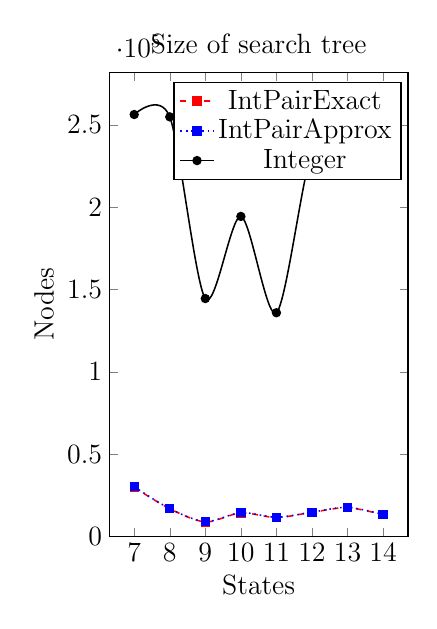
\begin{tikzpicture} [scale=0.7, font=\Large]
    \begin{axis}[
        title=Size of search tree,
        ylabel=Nodes,
        xtick=data,
        ymin=0, 
        xlabel=States ]
      \addplot[smooth,mark=square*, mark options={solid},red, dashed]
      coordinates{ (7,29788) (8,16760) (9,8770) (10,14248) (11,11456) (12,14602) (13,17456) (14,13112)
      }; \label{ie_plot} \addlegendentry{IntPairExact}
      \addplot[smooth,mark=square*, mark options={solid},blue, dotted]
      coordinates{ (7,30142) (8,16836) (9,8960) (10,14390) (11,11584) (12,14694) (13,17634) (14,13242)
      }; \label{ia_plot} \addlegendentry{IntPairApprox}
      \addplot[smooth,mark=*,mark options={solid},black]
      coordinates{ (7,256300) (8,254888) (9,144484) (10,194390) (11,135874) (12,233684) (13,243624) (14,221408)
      }; \label{int_plot} \addlegendentry{Integer}
    \end{axis}
  \end{tikzpicture}
  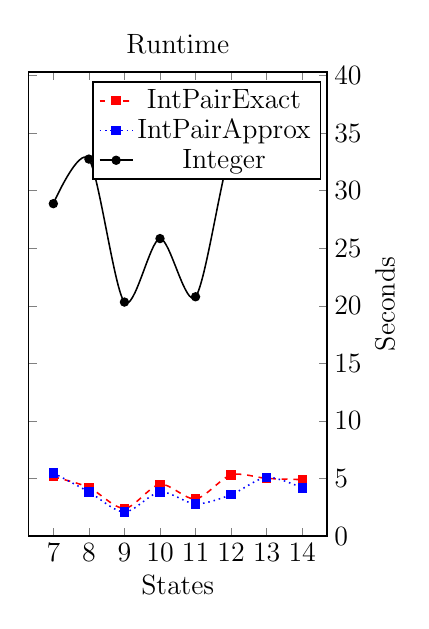
\begin{tikzpicture} [scale=0.7, font=\Large]
    \begin{axis}[
        yticklabel pos=right,
        xtick=data,
        title=Runtime,
        ylabel=Seconds,
        xlabel=States,
        ymin=0, ]
      \addplot[smooth,mark=square*,mark options={solid},red, dashed]
      coordinates{ (7, 5.146) (8, 4.220) (9, 2.397) (10, 4.500) (11, 3.223) (12, 5.308) (13, 5.009) (14, 4.901)
      }; \label{IntPairExact Run}
      \addplot[smooth,mark=square*,mark options={solid},blue, dotted]
      coordinates{ (7, 5.483) (8, 3.837) (9, 2.080) (10, 3.829) (11, 2.794) (12, 3.593) (13, 5.102) (14, 4.179)
      }; \label{IntPairApprox Run}
      \addplot[smooth,mark=*,mark options={solid},black]
      coordinates{ (7, 28.869) (8, 32.743) (9, 20.322) (10, 25.837) (11, 20.783) (12, 33.592) (13, 36.638) (14, 34.850)
      }; \label{IntegerRun}
      \addlegendentry{IntPairExact}
      \addlegendentry{IntPairApprox}
      \addlegendentry{Integer}
    \end{axis}
  \end{tikzpicture}

%  \begin{tikzpicture}[scale=1.4]
%    \draw[very thick] (-4,0) -- (4,0);
%    \draw[draw=white] (-5,-0.2) -- (5,-0.2);
%  \end{tikzpicture}


%  \begin{tikzpicture} [scale=0.7, font=\Large]
%    \begin{semilogyaxis}[
%        title=Size of search tree logarithmic scale,
%        ylabel=Nodes,
%        xtick=data,
%        ymin=0, 
%        xlabel=xlabel ]
%     \addplot[smooth,mark=square*, mark options={solid},red, dashed]
%      coordinates{ (7,29788) (8,16760) (9,8770) (10,14248) (11,11456) (12,14602) (13,17456) (14,13112)
%      }; \label{ie_plot} \addlegendentry{IntPairExact}
%      \addplot[smooth,mark=square*, mark options={solid},blue, dotted]
%      coordinates{ (7,30142) (8,16836) (9,8960) (10,14390) (11,11584) (12,14694) (13,17634) (14,13242)
%      }; \label{ia_plot} \addlegendentry{IntPairApprox}
%      \addplot[smooth,mark=*,mark options={solid},black]
%      coordinates{ (7,256300) (8,254888) (9,144484) (10,194390) (11,135874) (12,233684) (13,243624) (14,221408)
%      }; \label{int_plot} \addlegendentry{Integer}
%
%    \end{semilogyaxis}
%  \end{tikzpicture}
%  \begin{tikzpicture} [scale=0.7, font=\Large]
%    \begin{semilogyaxis}[
%        title=Runtime logaritmhic scale,
%        yticklabel pos=right,
%        xtick=data,
%        ylabel=Seconds,
%        xlabel=xlabel,
%        ymin=0,  ]
%      \addplot[smooth,mark=square*,mark options={solid},red, dashed]
%      coordinates{ (7, 5146) (8, 4220) (9, 2397) (10, 4500) (11, 3223) (12, 5308) (13, 5009) (14, 4901)
%      }; \label{IntPairExact Run}
%      \addplot[smooth,mark=square*,mark options={solid},blue, dotted]
%      coordinates{ (7, 5483) (8, 3837) (9, 2080) (10, 3829) (11, 2794) (12, 3593) (13, 5102) (14, 4179)
%      }; \label{IntPairApprox Run}
%      \addplot[smooth,mark=*,mark options={solid},black]
%      coordinates{ (7, 28869) (8, 32743) (9, 20322) (10, 25837) (11, 20783) (12, 33592) (13, 36638) (14, 34850)
%      }; \label{IntegerRun}
%      \addlegendentry{IntPairExact}
%      \addlegendentry{IntPairApprox}
%      \addlegendentry{Integer}
%    \end{semilogyaxis}
%  \end{tikzpicture}
  \caption{Varying the number of states. The other parameters are fixed: size of alphabet=10, max cost per transition=20, and number of steps=7.}\label{fig:states}
\end{figure}

\begin{figure}[H]
  \centering
  \textbf{Varying symbols }
  \newline
  \newline
  \pgfplotsset{
    scale only axis,
    legend style={at={(0,0.8)}, anchor=west, font=\tiny},
    xmin=7,
  }
  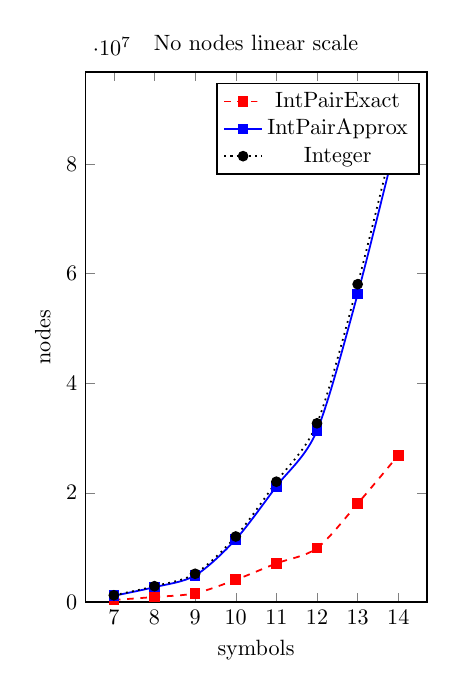
\begin{tikzpicture} [scale=0.8]
    \begin{axis}[
        title=No nodes linear scale,
        ylabel=nodes,
        xtick=data,
        ymin=0, 
        xlabel=symbols ]
      \addplot[smooth,mark=square*, mark options={solid},red, dashed]
      coordinates{ (7,427514) (8,969947) (9,1645581) (10,4116333) (11,7102695) (12,9882298) (13,18019942) (14,26841504)
      }; %\label{ie_plot}
      \addlegendentry{IntPairExact}
      \addplot[smooth,mark=square*, mark options={solid},blue]
      coordinates{ (7,1195984) (8,2764047) (9,4887805) (10,11496449) (11,21168309) (12,31364902) (13,56283604) (14,85763254)
      }; %\label{ia_plot}
      \addlegendentry{IntPairApprox}
      \addplot[smooth,mark=*,mark options={solid},black, dotted]
      coordinates{ (7,1283617) (8,2939856) (9,5206922) (10,12012764) (11,22020396) (12,32681442) (13,58068844) (14,88024314)
      }; %\label{int_plot}
      \addlegendentry{Integer}
    \end{axis}
  \end{tikzpicture}
  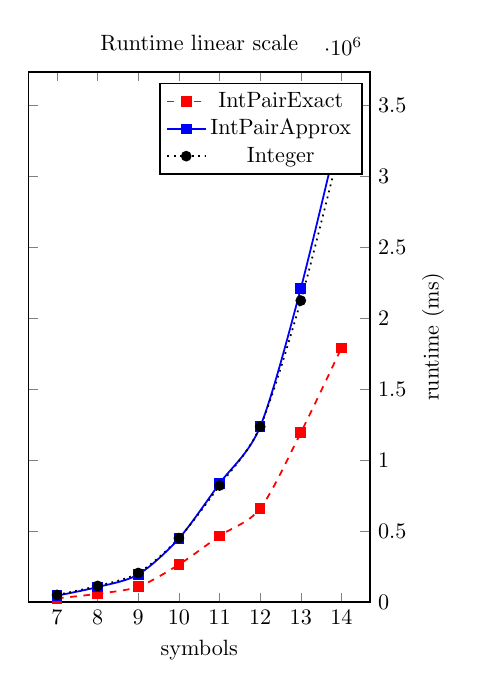
\begin{tikzpicture} [scale=0.8]
    \begin{axis}[
        yticklabel pos=right,
        xtick=data,
        title=Runtime linear scale,
        ylabel=runtime (ms),
        xlabel=symbols,
        ymin=0, ]
      \addplot[smooth,mark=square*,mark options={solid},red, dashed]
      coordinates{ (7, 27559) (8, 59866) (9, 109743) (10, 265565) (11, 467290) (12, 660466) (13, 1194665) (14, 1791396)
      };% \label{IntPairExact Run}
      \addplot[smooth,mark=square*,mark options={solid},blue]
      coordinates{ (7, 46890) (8, 107237) (9, 196052) (10, 449382) (11, 836755) (12, 1237011) (13, 2210994) (14, 3395879)
      }; %\label{IntPairApprox Run}
      \addplot[smooth,mark=*,mark options={solid},black, dotted]
      coordinates{ (7, 51783) (8, 115192) (9, 206274) (10, 452126) (11, 822169) (12, 1237290) (13, 2125013) (14, 3248002)
      }; %\label{IntegerRun}
      \addlegendentry{IntPairExact}
      \addlegendentry{IntPairApprox}
      \addlegendentry{Integer}
    \end{axis}
  \end{tikzpicture}

%  \begin{tikzpicture}[scale=1.4]
%    \draw[very thick] (-4,0) -- (4,0);
%    \draw[draw=white] (-5,-0.2) -- (5,-0.2);
%  \end{tikzpicture}


%  \begin{tikzpicture} [scale=0.8]
%    \begin{semilogyaxis}[
%        title=No nodes logarithmic scale,
%        ylabel=nodes,
%        xtick=data,
%        ymin=0, 
%        xlabel=symbols ]
%     \addplot[smooth,mark=square*, mark options={solid},red, dashed]
%      coordinates{ (7,427514) (8,969947) (9,1645581) (10,4116333) (11,7102695) (12,9882298) (13,18019942) (14,26841504)
%      }; %\label{ie_plot}
%      \addlegendentry{IntPairExact}
%      \addplot[smooth,mark=square*, mark options={solid},blue]
%      coordinates{ (7,1195984) (8,2764047) (9,4887805) (10,11496449) (11,21168309) (12,31364902) (13,56283604) (14,85763254)
%      }; %\label{ia_plot}
%      \addlegendentry{IntPairApprox}
%      \addplot[smooth,mark=*,mark options={solid},black, dotted]
%      coordinates{ (7,1283617) (8,2939856) (9,5206922) (10,12012764) (11,22020396) (12,32681442) (13,58068844) (14,88024314)
%      }; %\label{int_plot}
%      \addlegendentry{Integer}

%    \end{semilogyaxis}
%  \end{tikzpicture}
%  \begin{tikzpicture} [scale=0.8]
%    \begin{semilogyaxis}[
%        title=Runtime logaritmhic scale,
%        yticklabel pos=right,
%        xtick=data,
%        ylabel=runtime (ms),
%        xlabel=symbols,
%        ymin=0,  ]
%      \addplot[smooth,mark=square*,mark options={solid},red, dashed]
%      coordinates{ (7, 27559) (8, 59866) (9, 109743) (10, 265565) (11, 467290) (12, 660466) (13, 1194665) (14, 1791396)
%      }; %\label{IntPairExact Run}
%      \addplot[smooth,mark=square*,mark options={solid},blue]
%      coordinates{ (7, 46890) (8, 107237) (9, 196052) (10, 449382) (11, 836755) (12, 1237011) (13, 2210994) (14, 3395879)
%     }; %\label{IntPairApprox Run}
%      \addplot[smooth,mark=*,mark options={solid},black, dotted]
%      coordinates{ (7, 51783) (8, 115192) (9, 206274) (10, 452126) (11, 822169) (12, 1237290) (13, 2125013) (14, 3248002)
%      }; %\label{IntegerRun}
%      \addlegendentry{IntPairExact}
%      \addlegendentry{IntPairApprox}
%      \addlegendentry{Integer}
%    \end{semilogyaxis}
%  \end{tikzpicture}
  \caption{Varying the number of symbols. Other parameters are fixed. Number of states=7, max cost per transition=15 and number of steps=7.}\label{fig:symbols}
\end{figure}

\begin{figure}[H]
  \centering
  \textbf{Varying cost }
  \newline
  \newline
  \pgfplotsset{
    scale only axis,
    legend style={at={(0,0.8)}, anchor=west, font=\tiny},
    xmin=15,
  }
  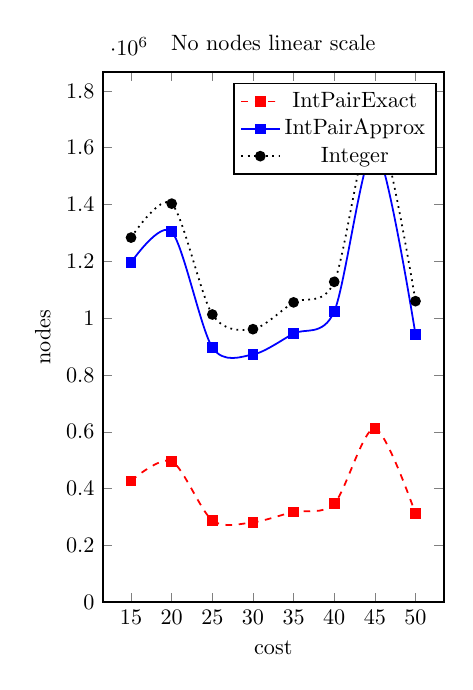
\begin{tikzpicture} [scale=0.8]
    \begin{axis}[
        title=No nodes linear scale,
        ylabel=nodes,
        xtick=data,
        ymin=0, 
        xlabel=cost ]
      \addplot[smooth,mark=square*, mark options={solid},red, dashed]
      coordinates{ (15,427514) (20,496441) (25,288296) (30,281590) (35,318147) (40,347192) (45,612036) (50,311950)
      }; %\label{ie_plot}
      \addlegendentry{IntPairExact}
      \addplot[smooth,mark=square*, mark options={solid},blue]
      coordinates{ (15,1195984) (20,1304175) (25,897266) (30,872190) (35,945941) (40,1023664) (45,1598498) (50,942876)
      }; %\label{ia_plot}
      \addlegendentry{IntPairApprox}
      \addplot[smooth,mark=*,mark options={solid},black, dotted]
      coordinates{ (15,1283617) (20,1403174) (25,1012948) (30,961248) (35,1055632) (40,1127914) (45,1696932) (50,1059848)
      }; %\label{int_plot}
      \addlegendentry{Integer}
    \end{axis}
  \end{tikzpicture}
  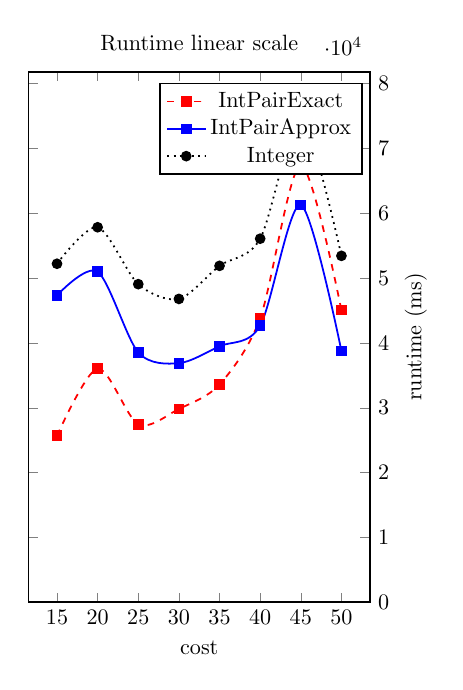
\begin{tikzpicture} [scale=0.8]
    \begin{axis}[
        yticklabel pos=right,
        xtick=data,
        title=Runtime linear scale,
        ylabel=runtime (ms),
        xlabel=cost,
        ymin=0, ]
      \addplot[smooth,mark=square*,mark options={solid},red, dashed]
      coordinates{ (15, 25684) (20, 36053) (25, 27456) (30, 29816) (35, 33596) (40, 43801) (45, 67417) (50, 45049)
      };% \label{IntPairExact Run}
      \addplot[smooth,mark=square*,mark options={solid},blue]
      coordinates{ (15, 47323) (20, 50981) (25, 38542) (30, 36873) (35, 39495) (40, 42646) (45, 61284) (50, 38757)
      }; %\label{IntPairApprox Run}
      \addplot[smooth,mark=*,mark options={solid},black, dotted]
      coordinates{ (15, 52210) (20, 57838) (25, 49062) (30, 46785) (35, 51887) (40, 56075) (45, 74353) (50, 53431)
      }; %\label{IntegerRun}
      \addlegendentry{IntPairExact}
      \addlegendentry{IntPairApprox}
      \addlegendentry{Integer}
    \end{axis}
  \end{tikzpicture}

%  \begin{tikzpicture}[scale=1.4]
%    \draw[very thick] (-4,0) -- (4,0);
%    \draw[draw=white] (-5,-0.2) -- (5,-0.2);
%  \end{tikzpicture}


%  \begin{tikzpicture} [scale=0.8]
%    \begin{semilogyaxis}[
%        title=No nodes logarithmic scale,
%        ylabel=nodes,
%        xtick=data,
%        ymin=0, 
%        xlabel=cost ]
%     \addplot[smooth,mark=square*, mark options={solid},red, dashed]
%      coordinates{ (15,427514) (20,496441) (25,288296) (30,281590) (35,318147) (40,347192) (45,612036) (50,311950)
%      }; %\label{ie_plot}
%      \addlegendentry{IntPairExact}
%      \addplot[smooth,mark=square*, mark options={solid},blue]
%      coordinates{ (15,1195984) (20,1304175) (25,897266) (30,872190) (35,945941) (40,1023664) (45,1598498) (50,942876)
%      }; %\label{ia_plot}
%      \addlegendentry{IntPairApprox}
%      \addplot[smooth,mark=*,mark options={solid},black, dotted]
%      coordinates{ (15,1283617) (20,1403174) (25,1012948) (30,961248) (35,1055632) (40,1127914) (45,1696932) (50,1059848)
%      }; %\label{int_plot}
%      \addlegendentry{Integer}

%    \end{semilogyaxis}
%  \end{tikzpicture}
%  \begin{tikzpicture} [scale=0.8]
%    \begin{semilogyaxis}[
%        title=Runtime logaritmhic scale,
%        yticklabel pos=right,
%        xtick=data,
%        ylabel=runtime (ms),
%        xlabel=cost,
%        ymin=0,  ]
%      \addplot[smooth,mark=square*,mark options={solid},red, dashed]
%      coordinates{ (15, 25684) (20, 36053) (25, 27456) (30, 29816) (35, 33596) (40, 43801) (45, 67417) (50, 45049)
%      }; %\label{IntPairExact Run}
%      \addplot[smooth,mark=square*,mark options={solid},blue]
%      coordinates{ (15, 47323) (20, 50981) (25, 38542) (30, 36873) (35, 39495) (40, 42646) (45, 61284) (50, 38757)
%     }; %\label{IntPairApprox Run}
%      \addplot[smooth,mark=*,mark options={solid},black, dotted]
%      coordinates{ (15, 52210) (20, 57838) (25, 49062) (30, 46785) (35, 51887) (40, 56075) (45, 74353) (50, 53431)
%      }; %\label{IntegerRun}
%      \addlegendentry{IntPairExact}
%      \addlegendentry{IntPairApprox}
%      \addlegendentry{Integer}
%    \end{semilogyaxis}
%  \end{tikzpicture}
%  \caption{{Caption}}\label{fig:}
\end{figure}

\begin{figure}[H]
  \centering
  \pgfplotsset{
    scaled y ticks=false,
    scale only axis,
    legend style={at={(0,0.8)}, anchor=west, font=\tiny},
    xmin=7,
  }
  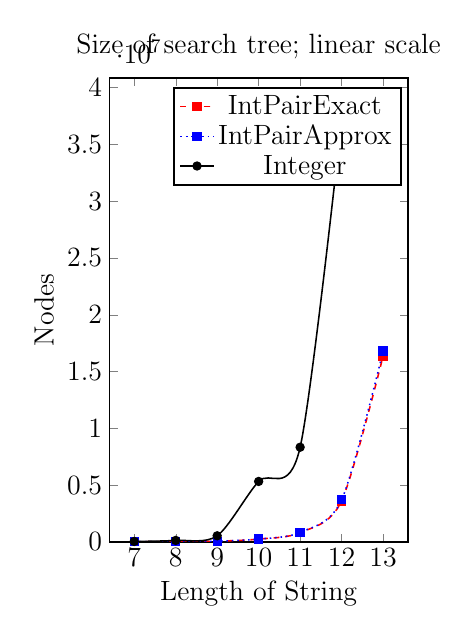
\begin{tikzpicture} [scale=0.7, font=\Large]
    \begin{axis}[
        title=Size of search tree; linear scale,
        ylabel=Nodes,
        xtick=data,
        ymin=0, 
        xlabel=Length of String ]
      \addplot[smooth,mark=square*, mark options={solid},red, dashed]
      coordinates{ (7,2958) (8,12299) (9,53945) (10,233801) (11,809042) (12,3602055) (13,16361867)
      }; \label{ie_plot} \addlegendentry{IntPairExact}
      \addplot[smooth,mark=square*, mark options={solid},blue, dotted]
      coordinates{ (7,3048) (8,12623) (9,55211) (10,240131) (11,829618) (12,3696025) (13,16790307)
      }; \label{ia_plot} \addlegendentry{IntPairApprox}
      \addplot[smooth,mark=*,mark options={solid},black]
      coordinates{ (7, 28628) (8, 121116) (9, 527254) (10, 5315546) (11, 8329154) (12, 37151208)
      }; \label{int_plot} \addlegendentry{Integer}
    \end{axis}
  \end{tikzpicture}
  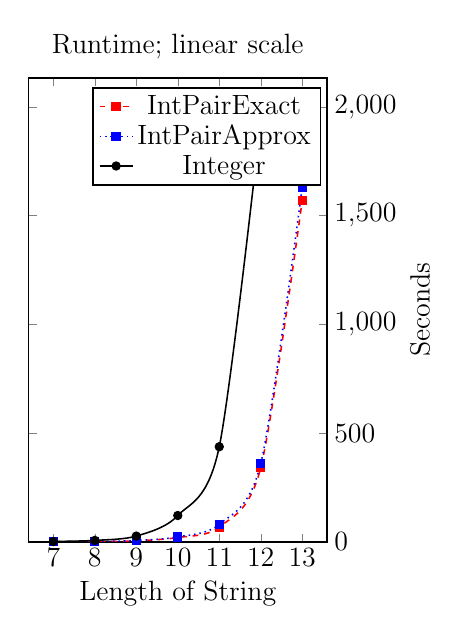
\begin{tikzpicture} [scale=0.7, font=\Large]
    \begin{axis}[
        yticklabel pos=right,
        xtick=data,
        title=Runtime; linear scale,
        ylabel=Seconds,
        xlabel=Length of String,
        ymin=0, ]
      \addplot[smooth,mark=square*,mark options={solid},red, dashed]
      coordinates{ (7, .339) (8, 1.142) (9, 4.601) (10, 19.534) (11, 67.852) (12, 340.757) (13, 1569.780)
      }; \label{IntPairExact Run}
      \addplot[smooth,mark=square*,mark options={solid},blue, dotted]
      coordinates{ (7, .290) (8, 1.263) (9, 5.724) (10, 22.607) (11, 80.168) (12, 359.915) (13, 1629.885)
      }; \label{IntPairApprox Run}
      \addplot[smooth,mark=*,mark options={solid},black]
      coordinates{ (7, 1.464) (8,6.312) (9, 26.246) (10, 120.832) (11, 437.171) (12, 1940.096)
      }; \label{IntegerRun}
      \addlegendentry{IntPairExact}
      \addlegendentry{IntPairApprox}
      \addlegendentry{Integer}
    \end{axis}
  \end{tikzpicture}

  
\begin{tikzpicture}[scale=1.4]
    \draw[very thick] (-4,0) -- (4,0);
    \draw[draw=white] (-5,-0.2) -- (5,-0.2);
  \end{tikzpicture}


  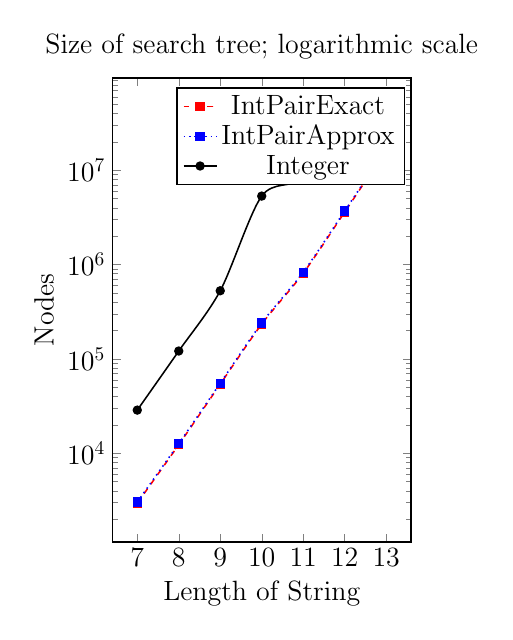
\begin{tikzpicture} [scale=0.7, font=\Large]
    \begin{semilogyaxis}[
        title=Size of search tree; logarithmic scale,
        ylabel=Nodes,
        xtick=data,
        ymin=0, 
        xlabel=Length of String ]
     \addplot[smooth,mark=square*, mark options={solid},red, dashed]
      coordinates{ (7,2958) (8,12299) (9,53945) (10,233801) (11,809042) (12,3602055) (13,16361867)
      }; \label{ie_plot} \addlegendentry{IntPairExact}
      \addplot[smooth,mark=square*, mark options={solid},blue, dotted]
      coordinates{ (7,3048) (8,12623) (9,55211) (10,240131) (11,829618) (12,3696025) (13,16790307)
      }; \label{ia_plot} \addlegendentry{IntPairApprox}
      \addplot[smooth,mark=*,mark options={solid},black]
      coordinates{ (7, 28628) (8, 121116) (9, 527254) (10, 5315546) (11, 8329154) (12, 37151208)
      }; \label{int_plot} \addlegendentry{Integer}

    \end{semilogyaxis}
  \end{tikzpicture}
  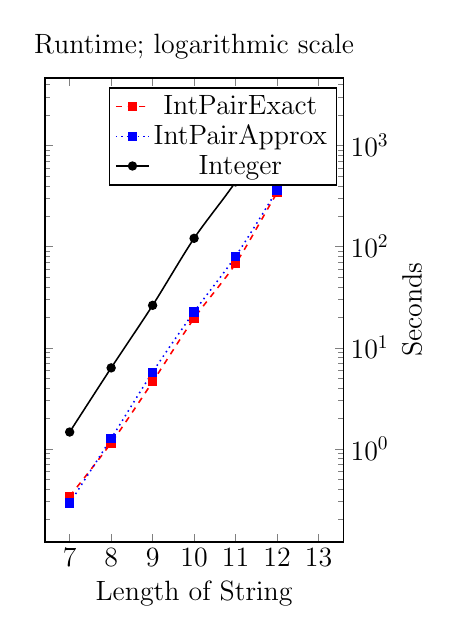
\begin{tikzpicture} [scale=0.7, font=\Large]
    \begin{semilogyaxis}[
        title=Runtime; logarithmic scale,
        yticklabel pos=right,
        xtick=data,
        ylabel=Seconds,
        xlabel=Length of String,
        ymin=0,  ]
      \addplot[smooth,mark=square*,mark options={solid},red, dashed]
      coordinates{ (7, .339) (8, 1.142) (9, 4.601) (10, 19.534) (11, 67.852) (12, 340.757) (13, 1569.780)
      }; \label{IntPairExact Run}
      \addplot[smooth,mark=square*,mark options={solid},blue, dotted]
      coordinates{ (7, .290) (8, 1.263) (9, 5.724) (10, 22.607) (11, 80.168) (12, 359.915) (13, 1629.885)
      }; \label{IntPairApprox Run}
      \addplot[smooth,mark=*,mark options={solid},black]
      coordinates{ (7, 1.464) (8,6.312) (9, 26.246) (10, 120.832) (11, 437.171) (12, 1940.096)
      }; \label{IntegerRun}
      \addlegendentry{IntPairExact}
      \addlegendentry{IntPairApprox}
      \addlegendentry{Integer}
    \end{semilogyaxis}
  \end{tikzpicture}
%  \input{}
%\end{figure}
  \caption{Varying the length of the string. The other parameters are fixed. Number of states=7, size of alphabet=7, and max cost per transition=15. Here we also show graphs in logarithmic scale. The integer variable timed out for $steps=13$.}\label{fig:steps}
 \end{figure}


%% symbols
\begin{figure}[H]
\centering
\textbf{Varying number of symbols}
\newline
\newline
	\pgfplotsset{
	    scale only axis,
		legend style={at={(0,0.8)}, anchor=west, font=\tiny},
	    xmin=5, xmax=8
	}
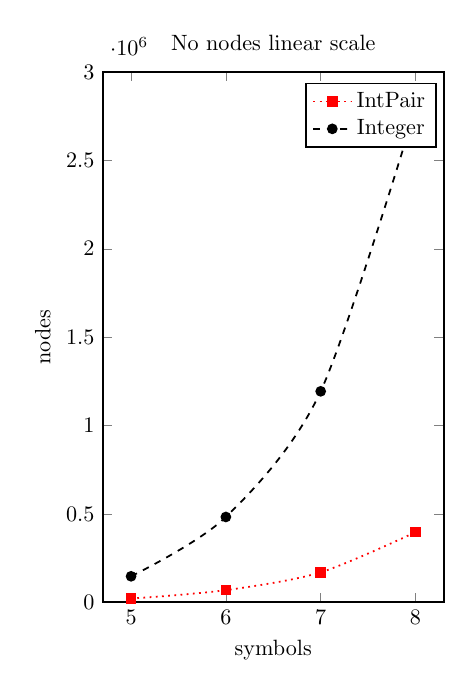
\begin{tikzpicture} [scale=0.8] 
	\begin{axis}[
		title=No nodes linear scale,
	  ylabel=nodes,
	  xtick=data,
  	  ymin=0, ymax=3000000,
  	  xlabel=symbols ]
		\addplot[smooth,mark=square*, mark options={solid},red, dotted]
		  coordinates{ (5,20879) (6,68523) (7,169435) (8,396625)
		}; \label{pnt_plot} \addlegendentry{IntPair}
		\addplot[smooth,mark=*,mark options={solid},black, dashed]
		  coordinates{ (5,146895) (6,482543) (7,1193363) (8,2791621)
		}; \label{int_plot} \addlegendentry{Integer}
	\end{axis}
\end{tikzpicture}
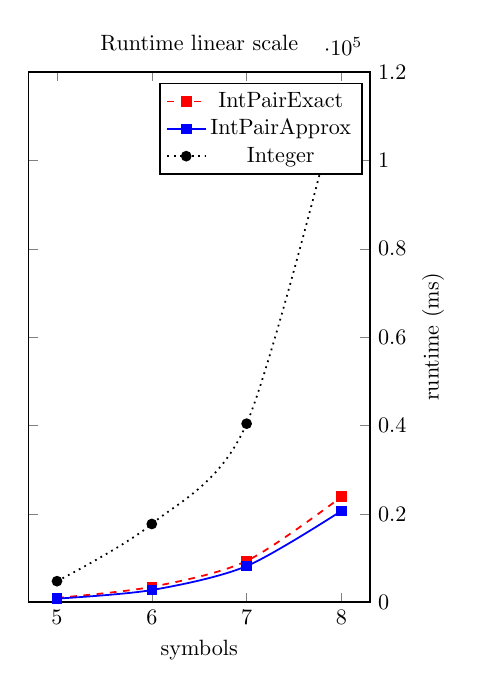
\begin{tikzpicture} [scale=0.8]
	\begin{axis}[
	yticklabel pos=right,
	  xtick=data,
		title=Runtime linear scale,
	  ylabel=runtime (ms),
  	 xlabel=symbols,
	  ymin=0, ymax=120000 ] 
		\addplot[smooth,mark=square*,mark options={solid},red, dashed]
		  coordinates{ (5,992) (6,3491) (7,9352) (8,23866)
		}; \label{IntPairExact Run}
		\addplot[smooth,mark=square*,mark options={solid},blue]
		  coordinates{ (5,827) (6,2767) (7,8186) (8,20679)
		}; \label{IntPairApprox Run}
		\addplot[smooth,mark=*,mark options={solid},black, dotted]
		  coordinates{ (5,4770) (6,17716) (7,40416) (8,116126)
		}; \label{IntegerRun}
		\addlegendentry{IntPairExact}
		\addlegendentry{IntPairApprox}
		\addlegendentry{Integer}
	\end{axis}
\end{tikzpicture}


\begin{tikzpicture}[scale=1.4]
\draw[very thick] (-4,0) -- (4,0);
\draw[draw=white] (-5,-0.2) -- (5,-0.2);
\end{tikzpicture}


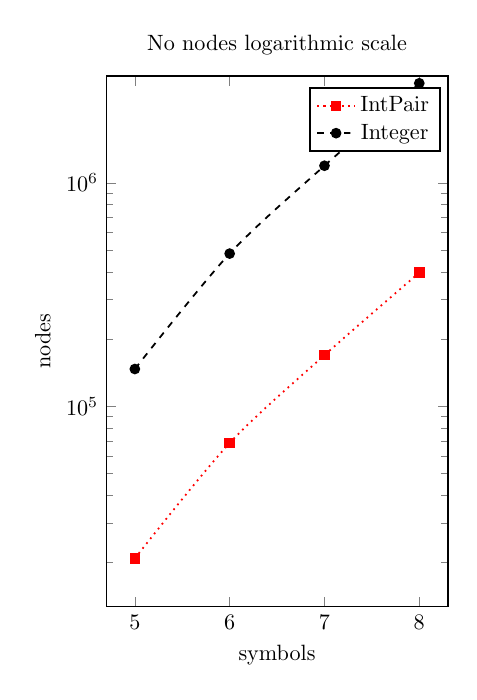
\begin{tikzpicture} [scale=0.8] 
	\begin{semilogyaxis}[
	  title=No nodes logarithmic scale,
	  ylabel=nodes,
	  xtick=data,
  	  ymin=0, ymax=3000000,
  	  xlabel=symbols ]
		\addplot[smooth,mark=square*, mark options={solid},red, dotted]
		  coordinates{ (5,20879) (6,68523) (7,169435) (8,396625)
		}; \label{pnt_plot} \addlegendentry{IntPair}
		\addplot[smooth,mark=*,mark options={solid},black, dashed]
		  coordinates{ (5,146895) (6,482543) (7,1193363) (8,2791621)
		}; \label{int_plot} \addlegendentry{Integer}
	\end{semilogyaxis}
\end{tikzpicture}
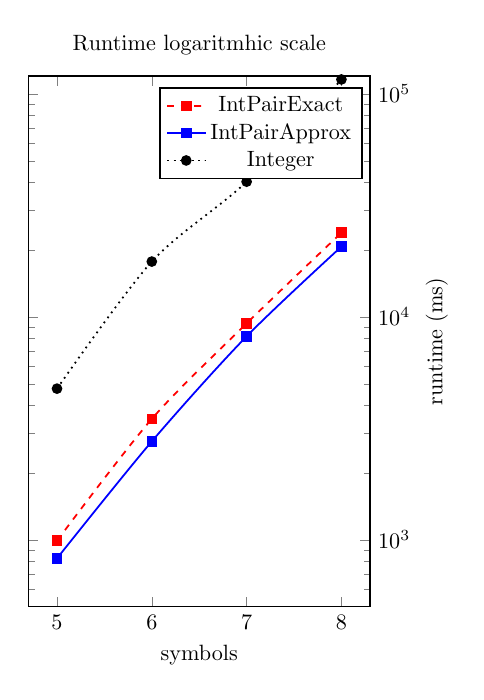
\begin{tikzpicture} [scale=0.8]
	\begin{semilogyaxis}[
		title=Runtime logaritmhic scale,
	yticklabel pos=right,
	  xtick=data,
	  ylabel=runtime (ms),
  	 xlabel=symbols,
	  ymin=0, ymax=120000 ] 
		\addplot[smooth,mark=square*,mark options={solid},red, dashed]
		  coordinates{ (5,992) (6,3491) (7,9352) (8,23866)
		}; \label{IntPairExact Run}
		\addplot[smooth,mark=square*,mark options={solid},blue]
		  coordinates{ (5,827) (6,2767) (7,8186) (8,20679)
		}; \label{IntPairApprox Run}
		\addplot[smooth,mark=*,mark options={solid},black, dotted]
		  coordinates{ (5,4770) (6,17716) (7,40416) (8,116126)
		}; \label{IntegerRun}
		\addlegendentry{IntPairExact}
		\addlegendentry{IntPairApprox}
		\addlegendentry{Integer}
	\end{semilogyaxis}
\end{tikzpicture}
\caption{{States=15, Maxcost=3, Steps=6}}\label{fig:symbols}
\end{figure}


%states
\begin{figure}[H]
\centering
\textbf{Varying number of states}
\newline
\newline
	\pgfplotsset{
	    scale only axis,
		legend style={at={(0,0.4)}, anchor=west, font=\tiny},
	    xmin=20, xmax=50
	}
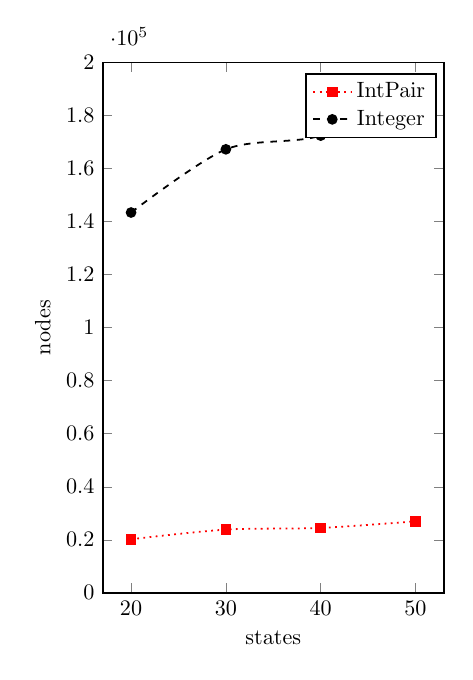
\begin{tikzpicture} [scale=0.8] 
	\begin{axis}[
	  ylabel=nodes,
	  xtick=data,
	  ymin=0, ymax=200000,
  	  xlabel=states ]
		\addplot[smooth,mark=square*, mark options={solid},red, dotted]
		  coordinates{ (20,20189) (30,23833) (40,24467) (50,26959)
		}; \label{pnt_plot} \addlegendentry{IntPair}
		\addplot[smooth,mark=*,mark options={solid},black, dashed]
		  coordinates{ (20,143413) (30,167251) (40,172417) (50,189809)
		}; \label{int_plot} \addlegendentry{Integer}
	\end{axis}
\end{tikzpicture}
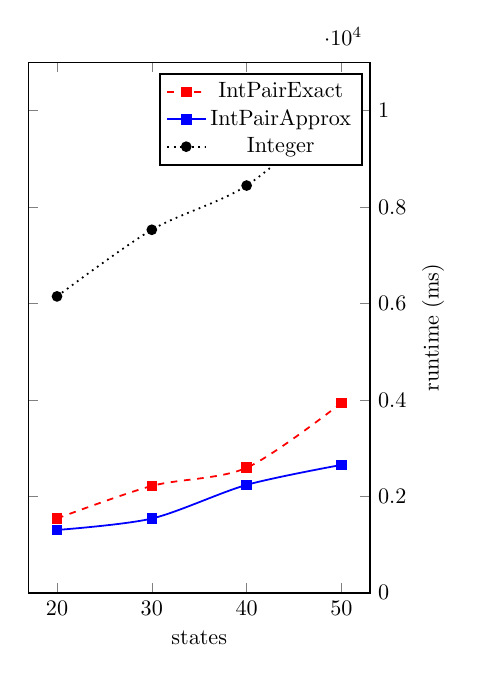
\begin{tikzpicture} [scale=0.8]
	\begin{axis}[
	yticklabel pos=right,
	  xtick=data,
	  ylabel=runtime (ms),
  	 xlabel=states,
	  ymin=0, ymax=11000 ] 
		\addplot[smooth,mark=square*,mark options={solid},red, dashed]
		  coordinates{ (20,1541)(30,2217)(40,2593) (50,3938)
		}; \label{IntPairExact Run}
		\addplot[smooth,mark=square*,mark options={solid},blue]
		  coordinates{ (20,1303) (30,1540) (40,2238) (50,2653)
		}; \label{IntPairApprox Run}
		\addplot[smooth,mark=*,mark options={solid},black, dotted]
		  coordinates{ (20,6148) (30,7530) (40,8447) (50,10086)
		}; \label{IntegerRun}
		\addlegendentry{IntPairExact}
		\addlegendentry{IntPairApprox}
		\addlegendentry{Integer}
	\end{axis}
\end{tikzpicture}
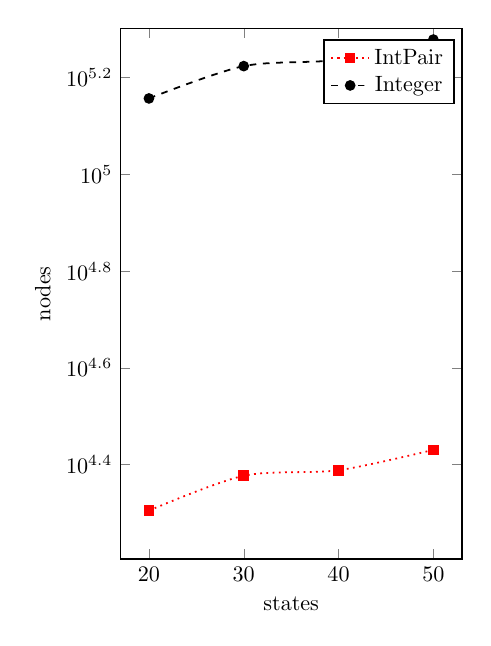
\begin{tikzpicture} [scale=0.8] 
	\begin{semilogyaxis}[
	  ylabel=nodes,
	  xtick=data,
	  ymin=0, ymax=200000,
  	  xlabel=states ]
		\addplot[smooth,mark=square*, mark options={solid},red, dotted]
		  coordinates{ (20,20189) (30,23833) (40,24467) (50,26959)
		}; \label{pnt_plot} \addlegendentry{IntPair}
		\addplot[smooth,mark=*,mark options={solid},black, dashed]
		  coordinates{ (20,143413) (30,167251) (40,172417) (50,189809)
		}; \label{int_plot} \addlegendentry{Integer}
	\end{semilogyaxis}
\end{tikzpicture}
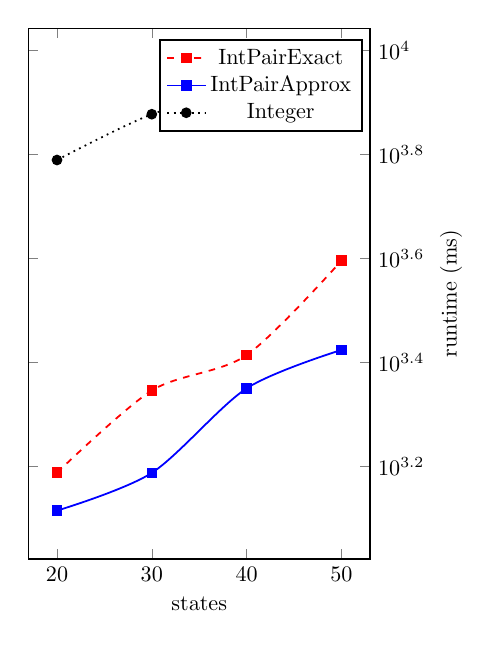
\begin{tikzpicture} [scale=0.8]
	\begin{semilogyaxis}[
	yticklabel pos=right,
	  xtick=data,
	  ylabel=runtime (ms),
  	 xlabel=states,
	  ymin=0, ymax=11000 ] 
		\addplot[smooth,mark=square*,mark options={solid},red, dashed]
		  coordinates{ (20,1541)(30,2217)(40,2593) (50,3938)
		}; \label{IntPairExact Run}
		\addplot[smooth,mark=square*,mark options={solid},blue]
		  coordinates{ (20,1303) (30,1540) (40,2238) (50,2653)
		}; \label{IntPairApprox Run}
		\addplot[smooth,mark=*,mark options={solid},black, dotted]
		  coordinates{ (20,6148) (30,7530) (40,8447) (50,10086)
		}; \label{IntegerRun}
		\addlegendentry{IntPairExact}
		\addlegendentry{IntPairApprox}
		\addlegendentry{Integer}
	\end{semilogyaxis}
\end{tikzpicture}
\caption{{Token=5, Maxcost=3, Steps=6}}\label{fig:states}
\end{figure}

%max cost
\begin{figure}[H]
\centering
\textbf{Varying maximum cost per transision}
\newline
\newline
	\pgfplotsset{
	    scale only axis,
		legend style={at={(0,0.4)}, anchor=west, font=\tiny},
	    xmin=2, xmax=15
	}
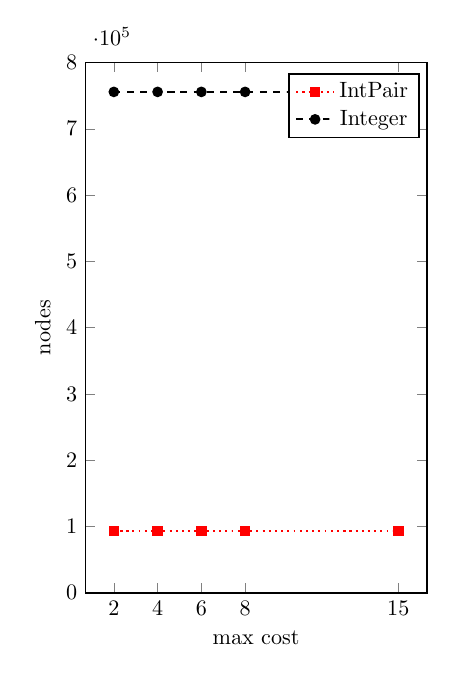
\begin{tikzpicture} [scale=0.8] 
	\begin{axis}[
	  ylabel=nodes,
	  xtick=data,
  	  ymin=2, ymax=800000,
  	  xlabel=max cost ]
		\addplot[smooth,mark=square*, mark options={solid},red, dotted]
		  coordinates{ (2,93227) (4,93227) (6,93227) (8,93227) (15,93227)
		}; \label{pnt_plot} \addlegendentry{IntPair}
		\addplot[smooth,mark=*,mark options={solid},black, dashed]
		  coordinates{ (2,755629) (4,755629) (6,755629) (8,755629) (15,755629)
		}; \label{int_plot} \addlegendentry{Integer}
	\end{axis}
\end{tikzpicture}
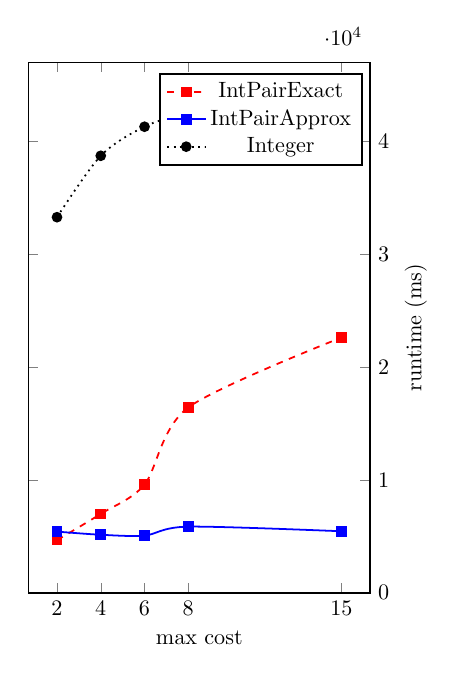
\begin{tikzpicture} [scale=0.8]
	\begin{axis}[
	yticklabel pos=right,
	  xtick=data,
	  ylabel=runtime (ms),
  	 xlabel=max cost,
	  ymin=0, ymax=47000 ] 
		\addplot[smooth,mark=square*,mark options={solid},red, dashed]
		  coordinates{ (2,4669) (4,6994) (6,9594) (8,16423) (15,22621)
		}; \label{IntPairExact Run}
		\addplot[smooth,mark=square*,mark options={solid},blue]
		  coordinates{ (2,5423) (4,5143)(6,5069) (8,5862) (15,5452)
		}; \label{IntPairApprox Run}
		\addplot[smooth,mark=*,mark options={solid},black, dotted]
		  coordinates{ (2,33288) (4,38731) (6,41307) (8,42426) (15,44868)
		}; \label{IntegerRun}
		\addlegendentry{IntPairExact}
		\addlegendentry{IntPairApprox}
		\addlegendentry{Integer}
	\end{axis}
\end{tikzpicture}
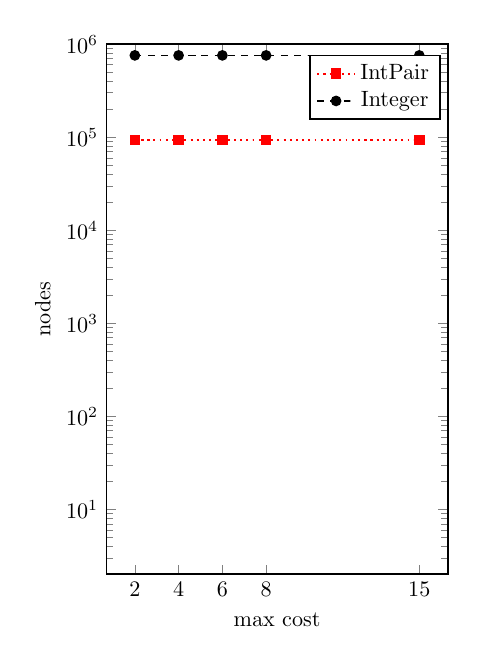
\begin{tikzpicture} [scale=0.8] 
	\begin{semilogyaxis}[
	  ylabel=nodes,
	  xtick=data,
  	  ymin=2, ymax=1000000,
  	  xlabel=max cost ]
		\addplot[smooth,mark=square*, mark options={solid},red, dotted]
		  coordinates{ (2,93227) (4,93227) (6,93227) (8,93227) (15,93227)
		}; \label{pnt_plot} \addlegendentry{IntPair}
		\addplot[smooth,mark=*,mark options={solid},black, dashed]
		  coordinates{ (2,755629) (4,755629) (6,755629) (8,755629) (15,755629)
		}; \label{int_plot} \addlegendentry{Integer}
	\end{semilogyaxis}
\end{tikzpicture}
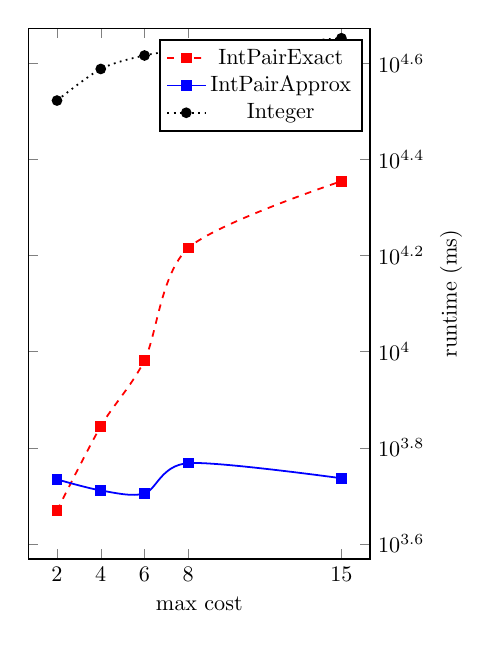
\begin{tikzpicture} [scale=0.8]
	\begin{semilogyaxis}[
	yticklabel pos=right,
	  xtick=data,
	  ylabel=runtime (ms),
  	 xlabel=max cost,
	  ymin=0, ymax=47000 ] 
		\addplot[smooth,mark=square*,mark options={solid},red, dashed]
		  coordinates{ (2,4669) (4,6994) (6,9594) (8,16423) (15,22621)
		}; \label{IntPairExact Run}
		\addplot[smooth,mark=square*,mark options={solid},blue]
		  coordinates{ (2,5423) (4,5143)(6,5069) (8,5862) (15,5452)
		}; \label{IntPairApprox Run}
		\addplot[smooth,mark=*,mark options={solid},black, dotted]
		  coordinates{ (2,33288) (4,38731) (6,41307) (8,42426) (15,44868)
		}; \label{IntegerRun}
		\addlegendentry{IntPairExact}
		\addlegendentry{IntPairApprox}
		\addlegendentry{Integer}
	\end{semilogyaxis}
\end{tikzpicture}
\caption{{Steps=20, Tokens=5, Steps=7. }}\label{fig:cost}
\end{figure}

%steps
\begin{figure}[H]
\centering
\textbf{Varying number of steps}
\newline
\newline

	\pgfplotsset{
	    scale only axis,
		legend style={at={(0,0.4)}, anchor=west, font=\tiny},
	    xmin=7, xmax=10
	}
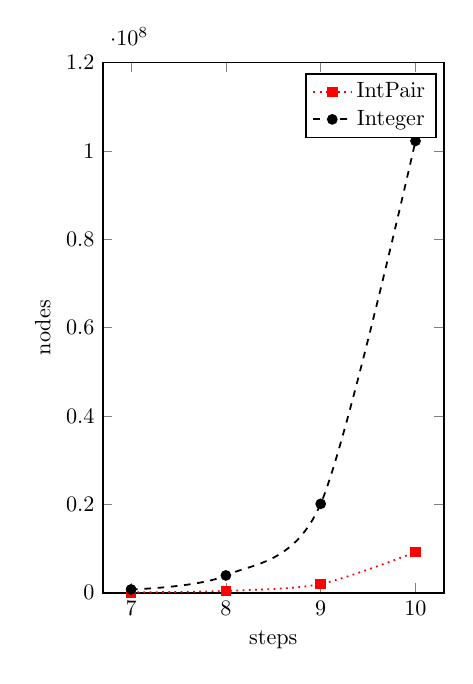
\begin{tikzpicture} [scale=0.8] 
	\begin{axis}[
	  ylabel=nodes,
	  xtick=data,
  	  ymin=2, ymax=120000000,
  	  xlabel=steps ]
		\addplot[smooth,mark=square*, mark options={solid},red, dotted]
		  coordinates{ (7,93227)  (8,431051) (9,1992011) (10,9207489)
		}; \label{pnt_plot} \addlegendentry{IntPair}
		\addplot[smooth,mark=*,mark options={solid},black, dashed]
		  coordinates{ (7,755629)(8,3924361)(9,20128261) (10,102243101)
		}; \label{int_plot} \addlegendentry{Integer}
	\end{axis}
\end{tikzpicture}
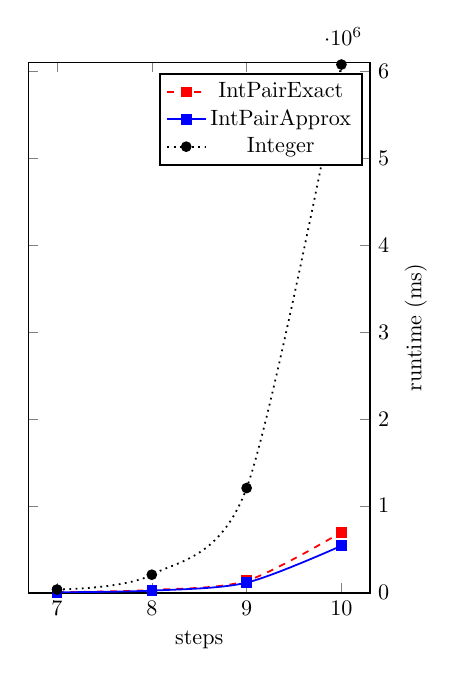
\begin{tikzpicture} [scale=0.8]
	\begin{axis}[
	yticklabel pos=right,
	  xtick=data,
	  ylabel=runtime (ms),
  	 xlabel=steps,
	  ymin=0, ymax=6100000] 
		\addplot[smooth,mark=square*,mark options={solid},red, dashed]
		  coordinates{ (7,6535) (8,32150) (9,137846) (10,696655)
		}; \label{IntPairExact Run}
		\addplot[smooth,mark=square*,mark options={solid},blue]
		  coordinates{ (7,5582)(8,24569)(9,116613) (10,540708)
		}; \label{IntPairApprox Run}
		\addplot[smooth,mark=*,mark options={solid},black, dotted]
		  coordinates{ (7,37169) (8,207591) (9,1204695)(10,6076224)
		}; \label{IntegerRun}
		\addlegendentry{IntPairExact}
		\addlegendentry{IntPairApprox}
		\addlegendentry{Integer}
	\end{axis}
\end{tikzpicture}
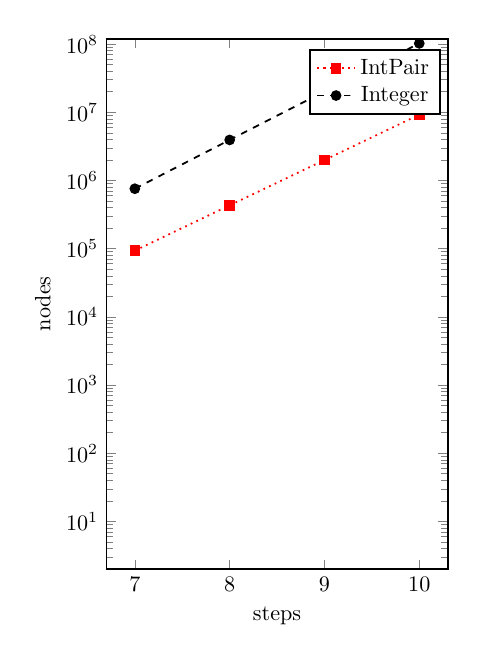
\begin{tikzpicture} [scale=0.8] 
	\begin{semilogyaxis}[
	  ylabel=nodes,
	  xtick=data,
  	  ymin=2, ymax=120000000,
  	  xlabel=steps ]
		\addplot[smooth,mark=square*, mark options={solid},red, dotted]
		  coordinates{ (7,93227)  (8,431051) (9,1992011) (10,9207489)
		}; \label{pnt_plot} \addlegendentry{IntPair}
		\addplot[smooth,mark=*,mark options={solid},black, dashed]
		  coordinates{ (7,755629)(8,3924361)(9,20128261) (10,102243101)
		}; \label{int_plot} \addlegendentry{Integer}
	\end{semilogyaxis}
\end{tikzpicture}
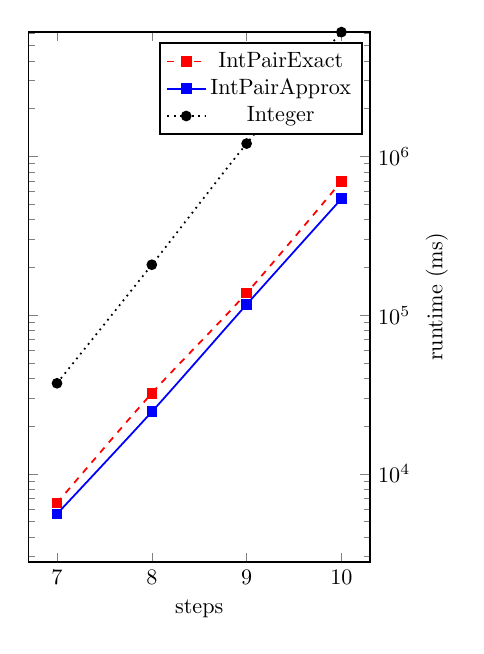
\begin{tikzpicture} [scale=0.8]
	\begin{semilogyaxis}[
	yticklabel pos=right,
	  xtick=data,
	  ylabel=runtime (ms),
  	 xlabel=steps,
	  ymin=0, ymax=6100000] 
		\addplot[smooth,mark=square*,mark options={solid},red, dashed]
		  coordinates{ (7,6535) (8,32150) (9,137846) (10,696655)
		}; \label{IntPairExact Run}
		\addplot[smooth,mark=square*,mark options={solid},blue]
		  coordinates{ (7,5582)(8,24569)(9,116613) (10,540708)
		}; \label{IntPairApprox Run}
		\addplot[smooth,mark=*,mark options={solid},black, dotted]
		  coordinates{ (7,37169) (8,207591) (9,1204695)(10,6076224)
		}; \label{IntegerRun}
		\addlegendentry{IntPairExact}
		\addlegendentry{IntPairApprox}
		\addlegendentry{Integer}
	\end{semilogyaxis}
\end{tikzpicture}
\caption{{States=20, Tokens=5, Maxcost=4}}\label{fig:steps}
\end{figure}

 


In the graphs we can see advantages for IntPairVar variables. In all tests they win over the regular IntVar variable solution in both execution time and the size of the search tree. However, it does so at the cost of higher memory usage per node. A node in the IntVar variable variant uses five IntVar variables, while the pair variants use two IntPair and one IntVar variable. The size of a node for the IntVar variable case should be roughly proportional to $Steps(States + Maxtotalcost)$ plus some overhead, but for the pair case the domain sizes of the pairs is proportional to the number of states times the max total cost. This means that the size per node is $Steps\times States\times Maxtotalcost$. For two-dimensional tuples with "normal" domain sizes this should not be of any concern. However, higher dimensions could cause trouble. The DFA problem could be modeled with a five-dimensional tuple variable. For the case in Figure~\ref{fig:states} with 50 states, 5 symbols, 6 steps and a maximum total cost of 18, the size per node would be around 100MB. Note though that the tuple variables have a higher memory usage \textit{per node} and that this does not necessarily mean that the total memory usage is higher, since the number of nodes shrinks. The case where the memory would be a problem is if the search tree became to deep, because a parent node can not be freed from memory until its children have been propagated to either a failure or a solution.

When tests were run (this is not shown in any graph) with the maximum total cost being equal to max cost per transition times the number of steps, the number of nodes is exactly equal for both IntPairExactVar and IntPairApproxVar. The reason is that if the starting state $s_0$ and the starting cumulative cost $c_0$ are assigned (which they are for a DFA), then everything else follows automatically if we branch on the symbols first. This is easy to see because $s_1=S(s_0, t_0)$ and $c_1=c_0+C(s_0, t_0)$. This is also confirmed by the fact that there were no failures during the execution. As can be seen in all graphs, this is not the case when restricting maximum total cost to a lower value.

In Figure~\ref{fig:steps}, the logarithmic graphs are close to straight lines. This indicates that all algorithms are exponential in both time and size of the search tree. Since the lines are parallel we can also see that they have the same exponential base. More importantly, this confirms that there was no complexity difference between tuple variables and IntVar variables when solving this problem. IntPairVar variables are faster, but not necessarily asymptotically faster. 

Figure~\ref{fig:states} and Figure~\ref{fig:cost} fluctuates very much. The difficulty of the problems does not seem to depend very much on the variable varied. When changing the number of states, the random generator generates completely different DFA:s. Changing the number of symbols also generate different DFA:s, but not in such a high degree. In the experiment there are one hundred random DFA:s for each measure point. Increasing this, would probably smoothen out the curve. The reason why the graphs for varying the cost per transition fluctuates so much is different. The maximum total cost is set to the maximum cost per transition times number of steps, so there are actually two parameters along the x-axis. One way to solve this would be to fix the maximum total cost to a fixed value. However, this is not a good solution, because a low value would make the problem easier when the cost per transition grows. On the other hand, a high value would make the problem to easy. This does not matter so much, since all the curves have the same shape, which means that if a DFA was hard to solve, it was hard for all three methods, making the comparison fair. 

All in all, the graphs indicate that tuple variables can give a better performance for certain problems. The only possible source of error with this experiment that I can think of is that the reference propagator may not be optimised enough, but I find that highly unlikely. After all, the implementation of IntVar has to be assumed to be very optimised, and the reference propagator is much more optimised than the ones for pairs.

\section{Related Work}
Beldiceanu et al. \cite{Beldiceanu675954} describes constraints for a counter-DFA (cDFA). It is defined as a regular DFA with only accepting states and such that the transition function not only returns the next state, but the increase for a counter. The DFA in this thesis is almost identical. The main difference is that we also use non-accepting states. The other difference is more philosophical. Instead of counting we talk about cost, but it makes no difference in practice. I wanted to do a performance comparison with that implementation, but it would be complicated to do that in a fair way, because the constraints are implemented in Prolog, while everything in this thesis is in C++.

Kellen Dye has implemented a bitvector for Gecode for her master thesis.\cite{Dye761927} That paper was useful for getting more understanding of how to implement a new variable in Gecode.

Monette et al.\cite{Monette771427} shows that tuple variables can be used to make pruning much more efficient. This thesis is basically a practical demonstration that this indeed is true, and that it translates into better performance.

\section{Conclusions and future work}
The tests shows that tuple variables have potential. Both of them perform better than the IntVar variable variant in both number of nodes and total execution time, and there is still much room for further improvement. Especially the vector operations are very inefficient and can easily be improved.

All big software libraries have coding standards. There is plenty of work to rewrite the code for IntPairVars in such a way that it satisfies Gecodes standards. For instance, vector from the standard library is not allowed. Furthermore, the code is far from ready in other aspects. It contains only the methods needed to run the tests in this thesis. One example of this is that it exists methods to get the minimum and maximum value for the first dimension, but no methods for the second. Also, the propagators and the brancher currently only accepts arrays. The brancher for IntPairApproxVar has a bug, which manifested itself by making the program producing the same solution several times which should not be possible. This does not matter in this thesis since it is not used.

In this thesis there is one exact and one approximate version. The approximation is exact in one dimension and only stores the boundaries for the second. This is just one way of doing it and there are several other ways of approximating the domain. Another relevant change that could be made is to extend the pairs to arbitrary dimensions.



\bibliographystyle{plain}
\bibliography{bib}
%\printbibliography

%\begin{btSect}[plain]{bibliography}
%\section*{References}
% \btPrintAll
%\end{btSect}

%\begin{thebibliography}{9}
%\bibitem{propreg}
%  Beldiceanu, Flener, Pearson, Van Hentenryck,
%  \emph{Propagating Regular Counting Constraints},
%
%\bibitem{bitvector}
%  Dye,
%  \emph{Implementation of bit-vector variables in a CP solver},
%
%\bibitem{propframe}
%  Monette, Flener, Pearson,
%  \emph{A propagator design framework for constraints over sequences},
%
%\bibitem{mpg}
%  Schulte, Tack, Lagerkvist
%  \emph{Modeling and Programming with Gecode},
%
%\end{thebibliography}
\end{document}
